\begin{savequote}[45mm]
\ascii{Any fool can write code that a computer can understand. Good programmers write code that humans can understand.}
\qauthor{\ascii{- Martin Flower}}
\end{savequote}

\chapter{分布式TensorFlow} 
\label{ch:distributed}

\begin{content}

\tf{}可以运行在分布式环境中,完成计算图的执行过程。本章将重点介绍 分布式运行时的基本架构与运行机制;重点讨论各个服务进程之间的交互关系;并且深入剖析在分布式环境中图操作,及其会话生命周期控制的关键技术;

\end{content}

\section{分布式模式}

\begin{content}

在分布式模式中,\ascii{Client}负责计算图的构造,然后通过调用\code{Session.run},启动计算图的执行过程。

\ascii{Master}进程收到计算图执行的消息后,启动计算图的剪枝,分裂,优化等操作;最终将子图分发注册到各个\ascii{Worker}进程上,然后触发各个\ascii{Worker}进程并发执行子图。

\ascii{Worker}进程收到子图注册的消息后,根据本地计算设备资源,再将计算子图实施二次分裂,将子图分配在各个计算设备上,最后启动各个计算设备并发地执行子图;如果\ascii{Worker}之间存在数据交换,可以通过进程间通信完成交互。

\begin{figure}[H]
\centering
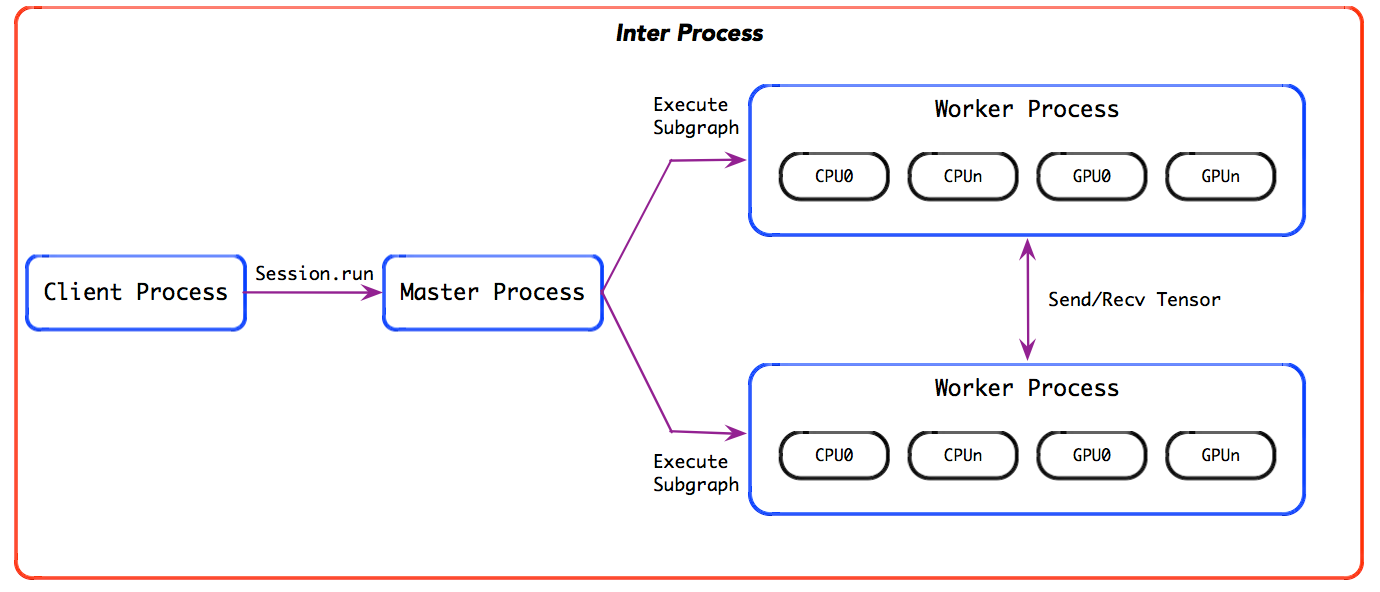
\includegraphics[width=0.8\textwidth]{figures/distributed.png}
\caption{分布式模式}
 \label{fig:distributed}
\end{figure}

\subsection{图操作}

如\refig{dist-runtime}所示,在\code{run\_step}执行过程之中,涉及计算图的剪枝、分裂、执行三个重要的图操作。其中,在分布式运行时,图分裂经历了两级分裂过程。

\begin{enum}
  \eitem{一级分裂:由\code{MasterSession}完成,按照\code{SplitByWorker}或\code{SplitByTask}完成图分裂过程;}
  \eitem{二级分裂:由\code{WorkerSession}完成,按照\code{SplitByDevice}完成图分裂过程。}
\end{enum}

在分布式模式中,图剪枝也体现了\tf{}部分执行的设计理念;而图分裂和执行也体现了\tf{}并发执行的设计理念。其中,图剪枝仅发生在\ascii{Master}上,不发生在\ascii{Worker}上;而图分裂发生在\ascii{Master}和\ascii{Worker}上;图执行仅仅发生在\ascii{Worker}上,不发生在\ascii{Master}上。

\begin{figure}[H]
\centering
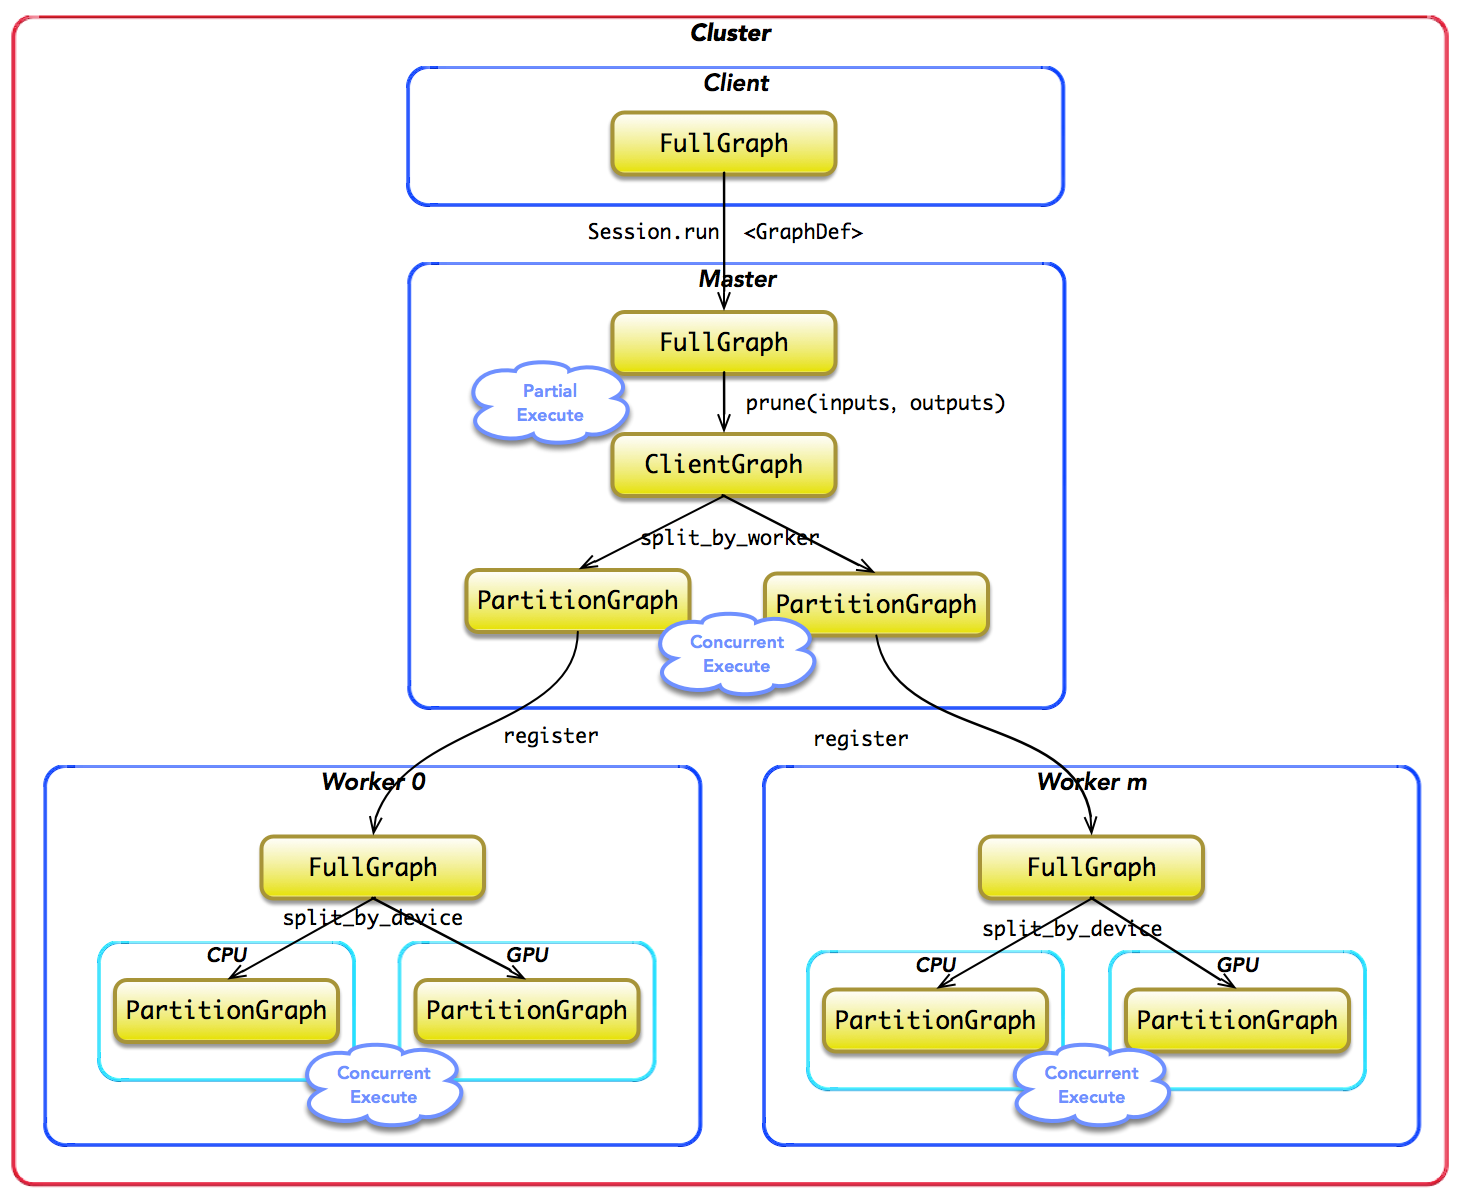
\includegraphics[width=1.0\textwidth]{figures/dist-runtime.png}
\caption{分布式:图操作}
 \label{fig:dist-runtime}
\end{figure}

\subsubsection{图分裂}

为了更好地理解分布式运行时的工作原理,以一个简单的例子阐述图操作的具体过程。如\refig{dist-exp-1}所示,假如存在一个简单的计算图,并且\code{f, c, a}部署在\code{/job:ps/task:0}上,且分别被编排到\code{CPU0, CPU1, CPU2}上;\code{g, h}部署在\code{/job:worker/task:0}上,且同时被编排到\code{GPU0}上;\code{b, d, e}部署在\code{/job:worker/task:1}上,且\code{d, e}被编排到\code{GPU0}上,而\code{b}被编排到\code{GPU1}上。

\begin{figure}[H]
\centering
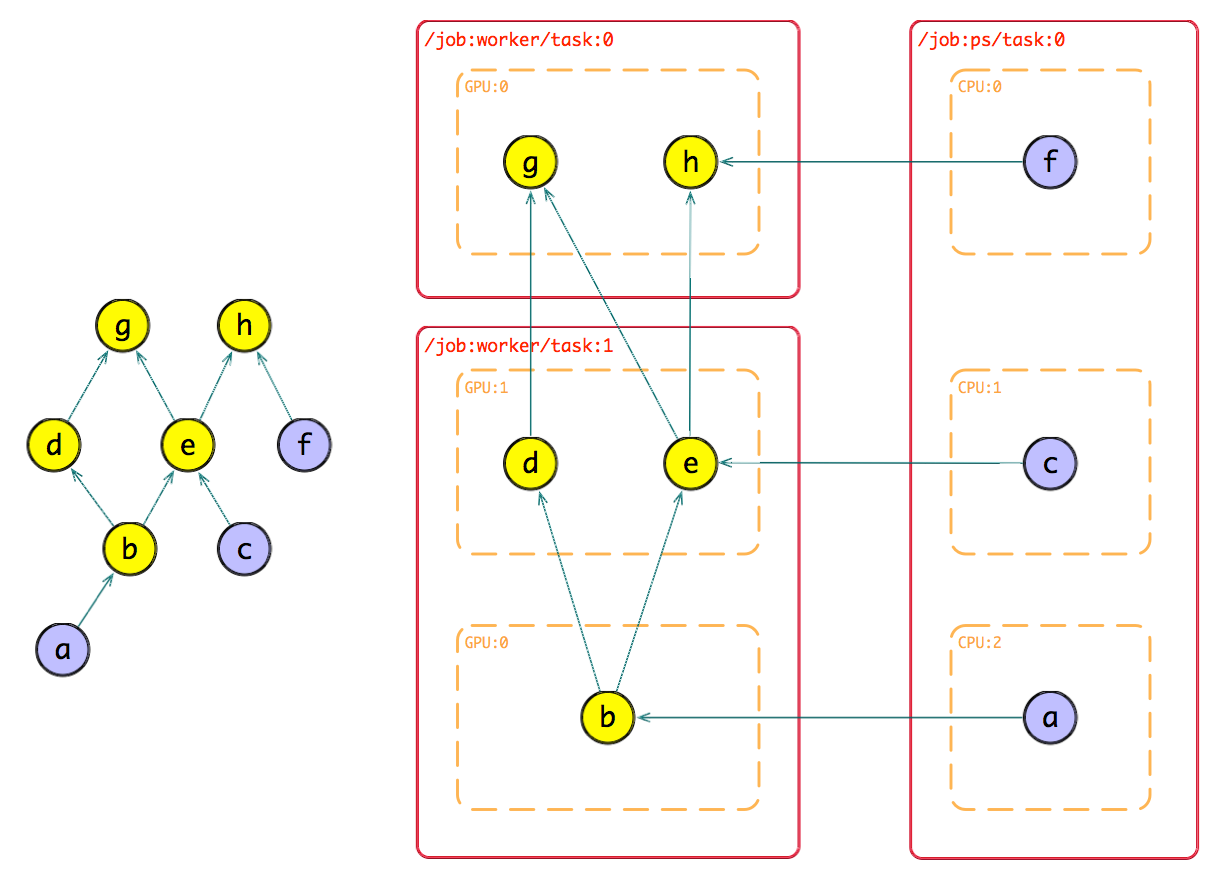
\includegraphics[width=1.0\textwidth]{figures/dist-exp-1.png}
\caption{分布式:图分裂}
 \label{fig:dist-exp-1}
\end{figure}

\subsubsection{数据交换}

如\refig{dist-exp-2}所示,对于跨设备的边,运行时自动实施边的分裂,分别在发送端和接收端插入\code{Send}和\code{Recv}两个末端节点。

进程间的\code{Send}和\code{Recv}节点,通过\code{GrpcRemoteRendezvous}实现数据交换。例如,\code{/job:ps/task:0}与\code{/job:worker/task:0},\code{/job:ps/task:0}与\code{/job:worker/task:1},或\code{/job:worker/task:0}与\code{/job:worker/task:1}之间是通过\code{GrpcRemoteRendezvous}完成数据交换的。

而进程内的\code{Send}和\code{Recv}节点,则通过\code{IntraProcessRendezvous}实现数据交换。例如,\code{/job:worker/task:1}内存在两个\code{GPU},它们之间采用\code{IntraProcessRendezvous}实现数据交换。

关于\code{Rendezvous}的具体实现过程,下文将还会重点讲述。

\begin{figure}[H]
\centering
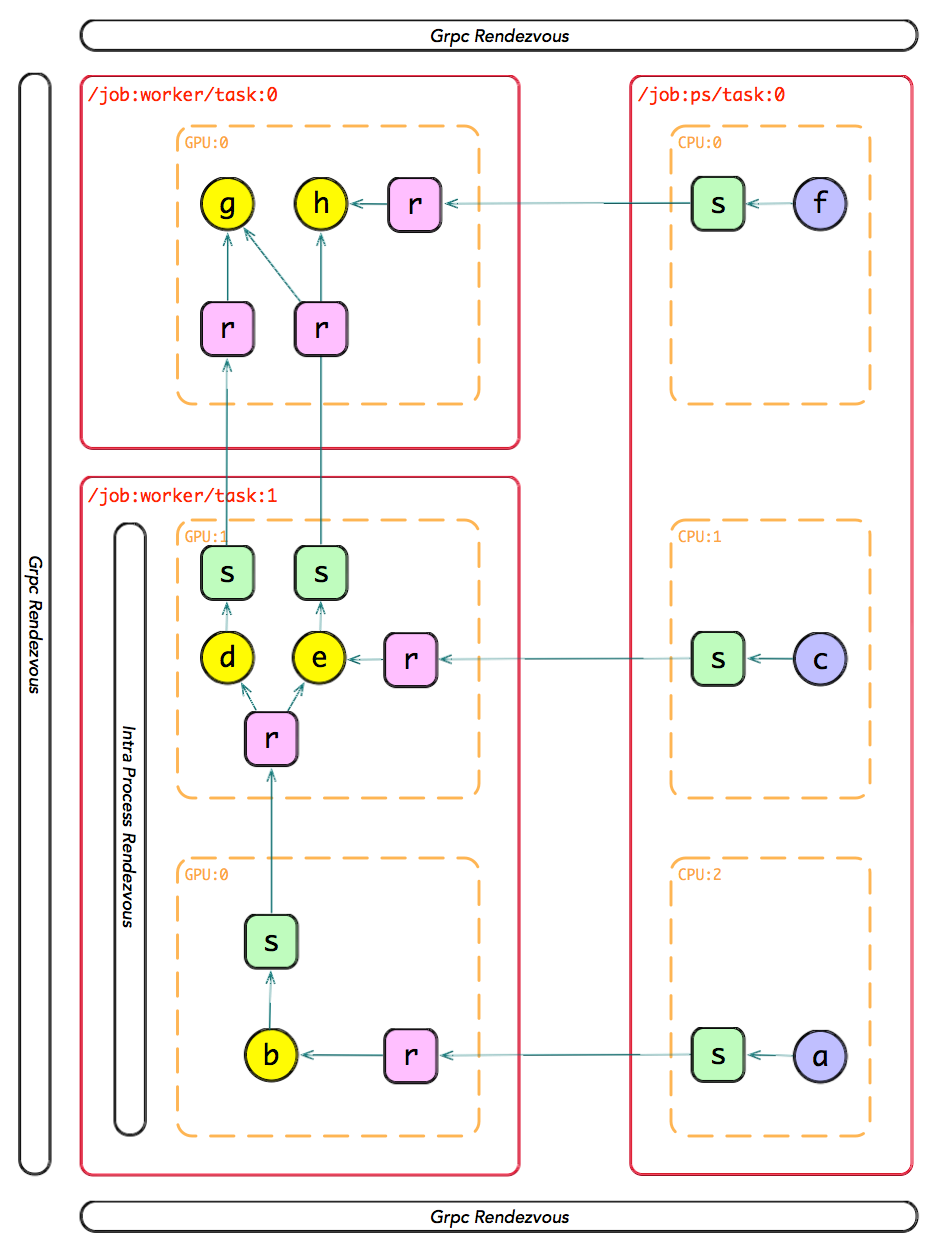
\includegraphics[width=0.8\textwidth]{figures/dist-exp-2.png}
\caption{分布式:数据交换}
 \label{fig:dist-exp-2}
\end{figure}

\subsection{领域模型}

如\refig{cc-dist-model}所示,在\tf{}分布式运行时,存在一个精巧的领域模型。

\begin{figure}[H]
\centering
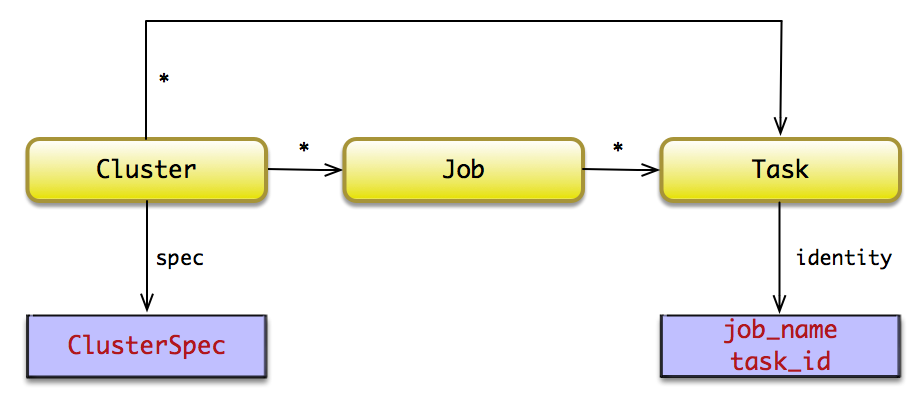
\includegraphics[width=0.7\textwidth]{figures/cc-dist-model.png}
\caption{分布式:领域模型}
 \label{fig:cc-dist-model}
\end{figure}

\subsubsection{Cluster}

\ascii{Cluster}使用\ascii{ClusterSpec}进行描述,它可以划分为一个或多个\ascii{Job},一个\ascii{Job}包含一个或多个\ascii{Task}。也就是说,\ascii{TensorFlow}集群是由执行计算图的任务集\ascii{(Task Set)}组成的。

每个\ascii{Task}可以独立运行在单独的机器上,也可以在一台机器上运行多个\ascii{Task}(例如,单机多\ascii{CPU},或单机多\ascii{GPU})。

\subsubsection{Job}

将目的相同的\ascii{Task}划归在同一个\ascii{Job}中。每个\ascii{Job}使用\code{job\_id}唯一标识。

一般地,在分布式深度学习的模型训练过程中,存在两种基本的\ascii{Job}类型:

\begin{enum}
  \eitem{\ascii{ps}:负责模型参数的存储和更新;}
  \eitem{\ascii{worker}:负责计算密集型的模型训练和推理。}
\end{enum}

\begin{figure}[H]
\centering
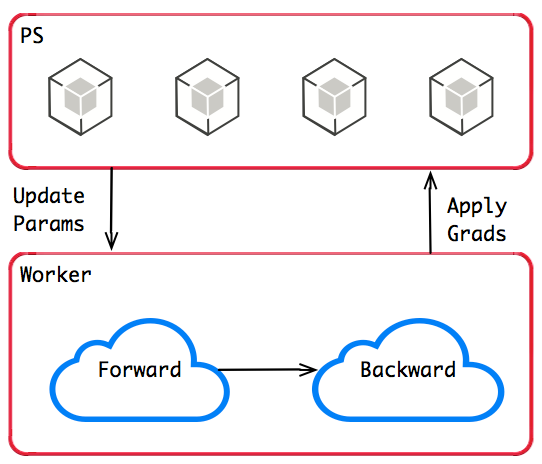
\includegraphics[width=0.5\textwidth]{figures/py-dist-ps-worker.png}
\caption{分布式模型训练:PS与Worker之间的交互}
 \label{fig:py-dist-ps-worker}
\end{figure}

\subsubsection{Task}

一般地,在分布式运行时中,\ascii{Task}运行在独立的进程中,并在其上运行一个\code{tf.train.Server}实例。其中,\ascii{Task}使用\code{job\_id:task\_index}的二元组唯一标识。

\subsubsection{Server}

\ascii{Server}表示\ascii{Task}的服务进程,它对外提供\code{MasterService}和\code{WorkerService}服务。也就是说,\ascii{Server}可以同时扮演\ascii{Master}和\ascii{Worker}两种角色。

\subsection{组建集群}

在分布式的\tf{}运行时中,每个\ascii{Task}启动了一个\ascii{Server},并对外提供\code{MasterService}服务和\code{WorkerService}服务。其中,组建\ascii{TensorFlow}集群包括两个基本步骤:

\begin{enum}
  \eitem{创建\code{tf.train.ClusterSpec},描述集群中\ascii{Task}的部署信息,并以\ascii{Job}的方式组织;}
  \eitem{对于每一个\ascii{Task},启动一个\code{tf.train.Server}实例。}
\end{enum}

\subsubsection{集群配置}

\code{ClusterSpec}描述了集群中\ascii{Task}的部署信息,并以\ascii{Job}的方式组织。一般地,在分布式的执行模式中,为每个\ascii{Task}启动一个进程。因此,\code{ClusterSpec}同时也描述了\ascii{TensorFlow}分布式运行时的进程分布情况。

例如,存在一个\ascii{TensorFlow}集群,它由\code{ps}和\code{worker}两个\ascii{Job}组成。其中,\code{ps}部署在\code{ps0:2222, ps1:2222}上;\code{worker}部署在\code{worker0:2222, worker1:2222, worker2:2222}上。

\begin{leftbar}
\begin{python}
tf.train.ClusterSpec({
  "worker": [
    "worker0:2222",   # /job:worker/task:0
    "worker1:2222",   # /job:worker/task:1
    "worker2:2222"    # /job:worker/task:2
  ],  
  "ps": [
    "ps0:2222",       # /job:ps/task:0
    "ps1:2222"        # /job:ps/task:0
  ]})
\end{python}
\end{leftbar}

在此例中,未显式地指定\ascii{Task}的索引。默认地,一个\ascii{Job}的\ascii{Task}集合中,\ascii{Task}索引从\ascii{0}开始按序自增的。

\subsubsection{Protobuf描述}

\begin{leftbar}
\begin{python}
message JobDef {
  string name = 1;
  map<int32, string> tasks = 2;
}

message ClusterDef {
  repeated JobDef job = 1;
}
\end{python}
\end{leftbar}

其中,\code{tasks}的关键字表示\code{task\_index},值表示\code{host:port}。

\end{content}

\section{服务器}

\begin{content}

\code{Server}是一个基于\ascii{gRPC}的服务器,负责管理本地设备集。它对外提供\code{MasterService}服务和\code{WorkerService}服务,具有同时扮演\ascii{Master}和\ascii{Worker}的角色。

\subsection{领域模型}

如\refig{cc-server-model}所示,\code{GrpcServer}扮演\ascii{Master}的角色时,对外提供\code{MasterService}服务;其中,它为每一个接入的\ascii{Client}启动一个\code{MasterSession}实例,并使用全局唯一的\code{session\_handle}标识它。也就是说,\ascii{Master}可以接入多个\ascii{Client},而一个\ascii{Client}则只能接入一个特定的\ascii{Master}。

\code{GrpcServer}扮演\ascii{Worker}的角色时,对外提供\code{WorkerService}服务;其中,每个\ascii{Worker}可以为多个\ascii{Master}提供计算服务,它为每个向它请求计算服务的\code{MasterSession}生成一个相应的\code{WorkerSession}实例,等待相应的\code{MasterSession}下发计算图的\emph{注册}和\emph{执行}命令。

整个\code{GrpcServer}实例承载于\code{grpc::Server}进程之上,它监听特定端口的消息,当消息到达时自动派发到\code{MasterService}或\code{WorkerService}中相应的消息处理的回调函数。

\begin{figure}[H]
\centering
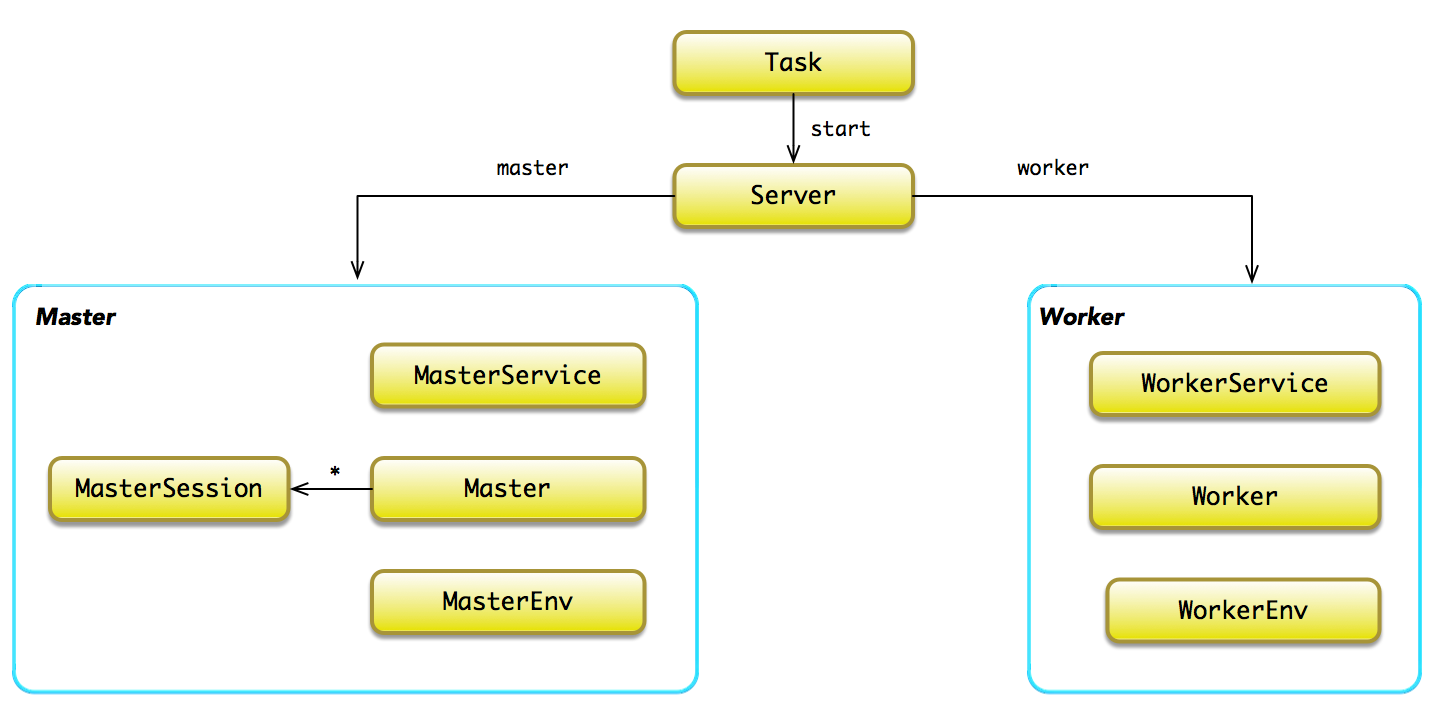
\includegraphics[width=1.0\textwidth]{figures/cc-server-model.png}
\caption{Server领域模型}
 \label{fig:cc-server-model}
\end{figure}

\subsubsection{Protobuf描述}

当\code{protocol}为\code{grpc}时,系统运行时将启用基于\ascii{gRPC}实现的\code{GrpcServer}实例。此外,可以通过\code{ConfigProto}实现运行时参数的配置。也就是说,\tf{}的架构是对外开放的。例如,通过扩展\code{protocol}支持新的通信协议,实现基于新协议的\code{Server}实例。

\begin{leftbar}
\begin{python}
message ServerDef {
  ClusterDef cluster = 1;
  
  string job_name = 2;
  int32 task_index = 3;

  ConfigProto default_session_config = 4;
  string protocol = 5;
}
\end{python}
\end{leftbar}

\subsubsection{服务互联}

如\refig{cc-server-interact}所示,一个\ascii{Server}实例通过\code{tf.train.ClusterSpec}与集群中的其他\ascii{Server}实例实现互联。

\begin{figure}[H]
\centering
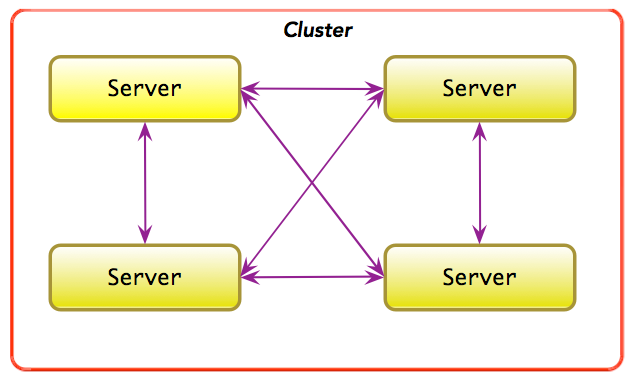
\includegraphics[width=0.5\textwidth]{figures/cc-server-interact.png}
\caption{服务互联}
 \label{fig:cc-server-interact}
\end{figure}

如\refig{cc-server-interact-1}所示,当\ascii{Client}接入其中一个\ascii{Server},此时它扮演了\ascii{Master}的角色,其他\ascii{Server}则扮演了\ascii{Worker}的角色。特殊地,\ascii{Client}接入的\ascii{Server}也扮演了\ascii{Worker}的角色。

\begin{figure}[H]
\centering
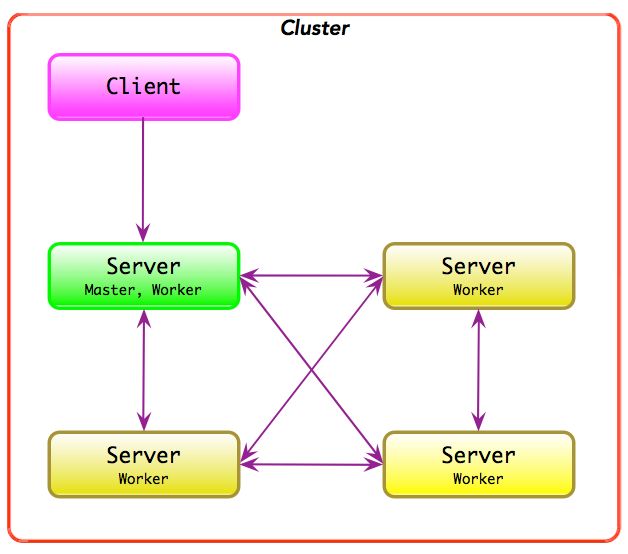
\includegraphics[width=0.5\textwidth]{figures/cc-server-interact-1.png}
\caption{单Client接入集群}
 \label{fig:cc-server-interact-1}
\end{figure}

如\refig{cc-server-interact-2}所示,可能存在多个\ascii{Client}分别接入不同的\ascii{Server}实例。此时,\ascii{Client}接入的\ascii{Server}实例扮演了\ascii{Master}角色。但是,该\ascii{Server}实例,相对于集群中另外的\ascii{Server}实例,则扮演了\ascii{Worker}角色。

\begin{figure}[H]
\centering
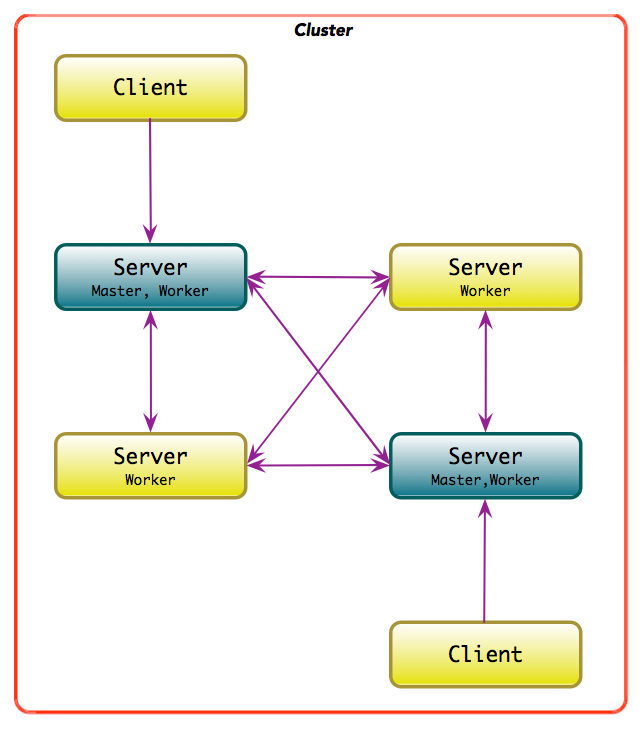
\includegraphics[width=0.5\textwidth]{figures/cc-server-interact-2.png}
\caption{多Client接入集群}
 \label{fig:cc-server-interact-2}
\end{figure}

特殊地,\ascii{Client}与\ascii{Master}可以部署在同一个进程内。此时,\ascii{Client}与\ascii{Master}之间的交互更加简单,两者直接使用函数调用,避免了\ascii{gRPC}交互的额外开销。依次类推,在同一个\ascii{Server}内,\ascii{Master}与\ascii{Worker}可以部署在同一进程内。此时,\ascii{Master}与\ascii{Worker}之间直接使用函数调用。

\subsection{状态机}

如\refig{dist-grpc-server-state-machine}所示,\code{GrpcServer}是一个基于\code{grpc::Server}的服务器,它管理和维护了一个简单的状态机。

\code{GrpcServer}在\code{New}状态上启动了\code{grpc::Server}服务,但对外并没有提供服务;而在\code{Started}状态上启动服务,对外提供\code{MasterService}和\code{WorkerService}的\code{RPC}消息服务;最终,在\code{Stopped}状态下停止\code{MasterService}和\code{WorkerService}服务。

\begin{figure}[H]
\centering
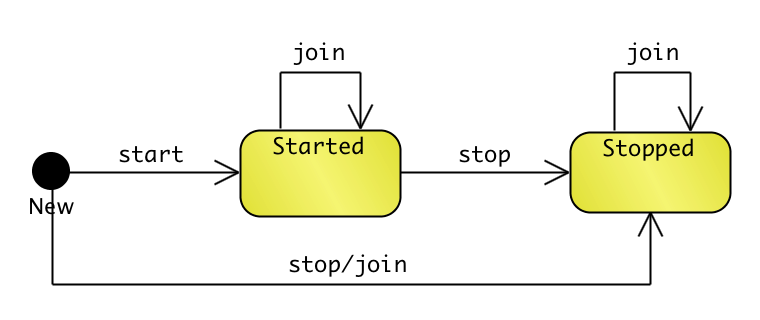
\includegraphics[width=0.7\textwidth]{figures/dist-grpc-server-state-machine.png}
\caption{GrpcServer状态机}
 \label{fig:dist-grpc-server-state-machine}
\end{figure}

\subsubsection{创建服务}

\begin{figure}[H]
\centering
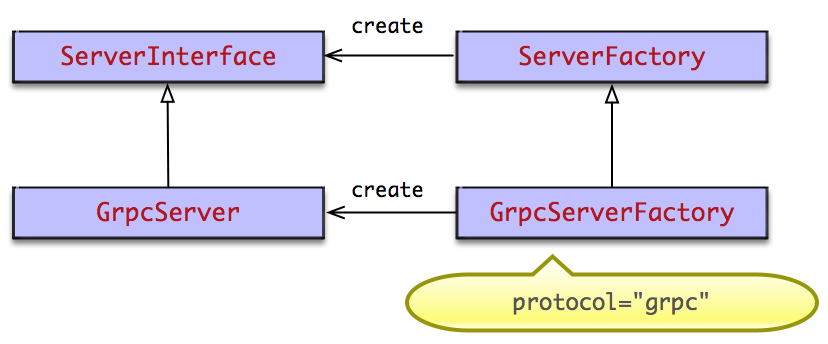
\includegraphics[width=0.7\textwidth]{figures/dist-grpc-server-factory.png}
\caption{多态创建Server实例}
 \label{fig:dist-grpc-server-factory}
\end{figure}

\begin{leftbar}
\begin{c++}
struct GrpcServerFactory : ServerFactory {
  bool AcceptsOptions(const ServerDef& server_def) override {
    return server_def.protocol() == "grpc";
  }

  Status NewServer(const ServerDef& server_def,
      std::unique_ptr<ServerInterface>* out_server) override {
    GrpcServer::Create(server_def, Env::Default(), out_server);
    return Status::OK();
  }
};
\end{c++}
\end{leftbar}

\begin{leftbar}
\begin{c++}
void GrpcServer::Create(
    const ServerDef& server_def, Env* env,
    std::unique_ptr<ServerInterface>* out_server) {
  auto ret = std::make_unique<GrpcServer>(server_def, env);
  ret->Init();
  *out_server = std::move(ret);
}
\end{c++}
\end{leftbar}

如\refig{cc-server-model}所示,\code{GrpcServer::Init}将完成\code{GrpcServer}领域对象的初始化,主要包括如下\ascii{3}个基本过程。

\begin{enum}
  \eitem{初始化\code{MasterEnv}实例;}  
  \eitem{初始化\code{WorkerEnv}实例;}  
  \eitem{创建并启动\code{grpc::Server}}    
    \begin{enum}
    \eitem{初始化\code{MasterService}}      
    \begin{nitemize}
      \eitem{创建\code{Master}实例;}  
      \eitem{创建\code{MasterService}实例;}
    \end{nitemize}
    \eitem{初始化\code{WorkerService}}          
    \begin{nitemize}          
      \eitem{创建\code{Worker}实例;}  
      \eitem{创建\code{WorkerService}实例。}
    \end{nitemize}      
    \end{enum}
\end{enum}

为了更好地理解整个\code{GrpcServer}实例的初始化过程,此处做了局部的重构。首先,它初始化\code{MasterEnv, WorkerEnv}实例;然后,创建并启动\code{grpc::Server}服务器。其中,初始化\code{MasterEnv/WorkerEnv},就是完成\code{MasterEnv/WorkerEnv}对象的构造过程,在此不再冗述。重点探究一下\code{grpc::Server}实例的构建和启动过程。

\begin{leftbar}
\begin{c++}
void GrpcServer::Init() {
  InitMasterEnv();
  InitWorkerEnv();
  StartGrpcServer();
}
\end{c++}
\end{leftbar}

实现使用构建器创建\code{grpc::Server}实例。首先,配置\code{grpc::Server}的服务选项;然后,分别构建\code{MasterService}实例和\code{WorkerService}实例。最后,调用\code{builder.BuildAndStart}方法启动\code{grpc::Server}服务器。

需要注意的是,\code{grpc::Server}启动时,\code{GrpcServer}依然处于\code{New}状态,
\code{grpc::Server}暂时还未对外提供\code{MasterService}服务和\code{WorkerService}服务。直至\code{GrpcServer}迁移至\code{Started}状态位置,\code{grpc::Server}才真正对外提供\code{MasterService}服务和\code{WorkerService}服务。

\begin{leftbar}
\begin{c++}
void InitServerBuilder(::grpc::ServerBuilder& builder) {
  builder.AddListeningPort(
    strings::StrCat("0.0.0.0:", GetRequestedPort()),
    GetServerCredentials(server_def_), &bound_port_);
  builder.SetMaxMessageSize(std::numeric_limits<int32>::max());
  builder.SetOption(
      std::unique_ptr<::grpc::ServerBuilderOption>(new NoReusePortOption));
}

void GrpcServer::StartGrpcServer() {
  ::grpc::ServerBuilder builder;

  InitServerBuilder(builder);
  InitMasterService(builder);
  InitWorkerService(builder);

  server_ = builder.BuildAndStart();  
}
\end{c++}
\end{leftbar}

很容易发现,\code{grpc::Server}对外提供\code{MasterService}服务的实体是\code{GrpcMasterService}实例。当消息到达时,将自动回调\code{GrpcMasterService}实例中相应的消息处理函数。其中,在消息处理函数中,其业务逻辑的处理完全依托于\code{Master}的领域对象。

\begin{leftbar}
\begin{c++}
std::unique_ptr<Master> GrpcServer::CreateMaster(
    MasterEnv* master_env) {
  return std::make_unique<Master>(master_env);
}

AsyncServiceInterface* NewGrpcMasterService(
    Master* master, ::grpc::ServerBuilder* builder) {
  return new GrpcMasterService(master, builder);
}

void GrpcServer::InitMasterService() {
  master_impl_ = CreateMaster(&master_env_);
  master_service_ = NewGrpcMasterService(
      master_impl_.get(), &builder);  
}
\end{c++}
\end{leftbar}

依次类推,\code{grpc::Server}对外提供\code{WorkerService}服务的实体是\code{GrpcWorkerService}实例。当消息到达时,将自动回调\code{GrpcWorkerService}实例中相应的消息处理函数。其中,在消息处理函数中,其业务逻辑的处理完全依托于\code{GrpcWorker}的领域对象。

\begin{leftbar}
\begin{c++}
std::unique_ptr<GrpcWorker> NewGrpcWorker(WorkerEnv* env) {
  return std::unique_ptr<GrpcWorker>(new GrpcWorker(env));
}

AsyncServiceInterface* NewGrpcWorkerService(
    GrpcWorker* worker, ::grpc::ServerBuilder* builder) {
  return new GrpcWorkerService(worker, builder);
}

void GrpcServer::InitWorkerService(::grpc::ServerBuilder& builder) {
  worker_impl_ = NewGrpcWorker(&worker_env_);
  worker_service_ = NewGrpcWorkerService(
    worker_impl_.get(), &builder);
}
\end{c++}
\end{leftbar}

\subsubsection{启动服务}

在\code{New}状态,\code{grpc::Server}已经启动,但暂时没有对外提供\code{MasterService}服务和\code{WorkerService}服务。通过调用\code{GrpcServer::Start}方法后,\code{GrpcServer}的状态从\code{New}迁移\code{Started}状态,并启动了两个独立的线程,分别启动\code{MasterService}和\code{WorkerService}的消息处理器。此时,\code{GrpcServer}正式对外提供\code{MasterService}和\code{WorkerService}。

\begin{leftbar}
\begin{c++}
Status GrpcServer::Start() {
  mutex_lock l(mu_);
  switch (state_) {
    case NEW: {
      master_thread_.reset(
          env_->StartThread(ThreadOptions(), "TF_master_service",
                            [this] { master_service_->HandleRPCsLoop(); }));
      worker_thread_.reset(
          env_->StartThread(ThreadOptions(), "TF_worker_service",
                            [this] { worker_service_->HandleRPCsLoop(); }));
      state_ = STARTED;
      return Status::OK();
    }
    case STARTED:
      LOG(INFO) << "Server already started(" << target() << ")";    
      return Status::OK();
    case STOPPED:
    default:
      CHECK(false);
  }
}
\end{c++}
\end{leftbar}

\subsubsection{等待终止服务}

为了持久地对外提供\code{MasterService}服务和\code{WorkerService}服务,需要分别对线程\code{TF\_master\_service}和\code{TF\_worker\_service}实施\code{join}操作,使得主线程挂起,直至这两个线程终止。

通过调用\code{GrpcServer::Join}方法,当\code{GrpcServer}处于\code{Started}或\code{Stoped}状态时,它将自动调用\code{Thread}的析构函数。

\begin{leftbar}
\begin{c++}
Status GrpcServer::Join() {
  mutex_lock l(mu_);
  switch (state_) {
    case NEW:
      // Prevent the server from being started subsequently.
      state_ = STOPPED;
      return Status::OK();
    case STARTED:
    case STOPPED:
      master_thread_.reset();
      worker_thread_.reset();
      return Status::OK();
    default:
      CHECK(false);
  }
}
\end{c++}
\end{leftbar}

例如,基于\code{C++}标准库实现的\code{StdThread}中,其析构函数将调用\code{std::thread}的\code{join}方法。

\begin{leftbar}
\begin{c++}
struct StdThread : Thread {
  StdThread(const ThreadOptions&, const string&, 
      std::function<void()> fn)
    : thread_(fn) {
  }

  ~StdThread() override { 
    thread_.join(); 
  }

 private:
  std::thread thread_;
};
\end{c++}
\end{leftbar}

\subsubsection{终止服务}

遗憾的是,目前\code{GrpcServer}并不能优雅地退出。因此,在工程实践环境中,\tf{}的分布式运行时常常需要借助于\code{Kubernetes},实现\code{GrpcServer}服务的自动管理。

\begin{leftbar}
\begin{c++}
Status GrpcServer::Stop() {
  mutex_lock l(mu_);
  switch (state_) {
    case NEW:
      state_ = STOPPED;
      return Status::OK();
    case STARTED:
      return errors::Unimplemented(
          "Clean shutdown is not currently implemented");
    case STOPPED:
      LOG(INFO) << "Server already stopped(" << target() << ")";
      return Status::OK();
    default:
      CHECK(false);
  }
}
\end{c++}
\end{leftbar}

\section{Master服务}

\begin{content}

\code{MasterService}是一个\ascii{RPC}服务。当\ascii{Client}根据\code{target}接入\ascii{Server}实例后,\ascii{Server}扮演了\ascii{Master}的角色,对外提供\code{MasterService}服务。

其中,\ascii{Client}与\ascii{Master}之间的交互遵循\code{MasterService}定义的接口规范。也就是说,\code{MasterService}定义了\ascii{Client}接入\ascii{Master}的公共契约,负责协调和控制多个\code{WorkerService}的执行过程。

\subsection{接口定义}

在\code{master\_service.proto}文件中,定义了\code{MasterService}的所有接口;而在\code{master.proto}文件中,定义了各个接口的消息体。

\begin{leftbar}
\begin{c++}
service MasterService {
  rpc CreateSession(CreateSessionRequest) 
      returns (CreateSessionResponse);
  
  rpc ExtendSession(ExtendSessionRequest) 
      returns (ExtendSessionResponse);

  rpc PartialRunSetup(PartialRunSetupRequest) 
      returns (PartialRunSetupResponse);

  rpc RunStep(RunStepRequest) 
      returns (RunStepResponse);
  
  rpc CloseSession(CloseSessionRequest) 
      returns (CloseSessionResponse);
  
  rpc ListDevices(ListDevicesRequest) 
      returns (ListDevicesResponse);

  rpc Reset(ResetRequest) 
      returns (ResetResponse);
}
\end{c++}
\end{leftbar}

\subsection{访问服务}

一般地,\ascii{Client}使用接口\code{MasterInterface}获取远端\code{MasterService}的服务。特殊地,\code{MasterInterface}的所有接口都是同步接口,使得\ascii{Client}访问远端\code{MasterService}服务犹如调用本地函数一般。

需要注意的是,因为\code{RunStepRequest/RunStepResponse}消息中可能包含较大的\code{Tensor}实例。为了避免不必要的对象拷贝,实现特化实现了消息包装器。

\begin{leftbar}
\begin{c++}
// Abstract interface for communicating with the TensorFlow Master service.
//
// This interface supports both RPC-based master implementations, and
// in-process master implementations that do not require an RPC roundtrip.
struct MasterInterface {
  virtual ~MasterInterface() {}
  
  virtual Status CreateSession(
      CallOptions* call_options,
      const CreateSessionRequest* request,
      CreateSessionResponse* response) = 0;

  virtual Status ExtendSession(
      CallOptions* call_options,
      const ExtendSessionRequest* request,
      ExtendSessionResponse* response) = 0;

  virtual Status PartialRunSetup(
      CallOptions* call_options,
      const PartialRunSetupRequest* request,
      PartialRunSetupResponse* response) {
    return errors::Unimplemented(
      "Partial run not implemented for master");
  }

  virtual Status RunStep(
      CallOptions* call_options,
      RunStepRequestWrapper* request,
      MutableRunStepResponseWrapper* response) = 0;

  // Wrapper classes for the `MasterService.RunStep` message.
  //
  // The `RunStepRequest/RunStepResponse` message can contain 
  // potentially large tensor data as part of its `feed/fetch` 
  // submessages.
  virtual Status RunStep(
    CallOptions* call_options,
    const RunStepRequest* request,
    RunStepResponse* response) {
    std::unique_ptr<RunStepRequestWrapper> wrapped_request(
        new ProtoRunStepRequest(request));
    std::unique_ptr<MutableRunStepResponseWrapper> wrapped_response(
        new NonOwnedProtoRunStepResponse(response));
    return RunStep(call_options, 
        wrapped_request.get(), 
        wrapped_response.get());
  }

  // Returns a request object for use in calls to
  // `RunStep()`. Ownership is transferred to the caller.
  virtual MutableRunStepRequestWrapper* CreateRunStepRequest() {
    return new MutableProtoRunStepRequest;
  }

  // Returns a response object for use in calls to
  // `RunStep()`. Ownership is transferred to the caller.
  virtual MutableRunStepResponseWrapper* CreateRunStepResponse() {
    return new OwnedProtoRunStepResponse;
  }

  virtual Status CloseSession(
    CallOptions* call_options,
    const CloseSessionRequest* request,
    CloseSessionResponse* response) = 0;

  virtual Status ListDevices(
    CallOptions* call_options,
    const ListDevicesRequest* request,
    ListDevicesResponse* response) = 0;

  virtual Status Reset(
    CallOptions* call_options, const ResetRequest* request,
    ResetResponse* response) = 0;
};
\end{c++}
\end{leftbar}

如\refig{dist-master-interface}所示,\code{MasterInterface}存在两种基本实现。

\begin{enum}
  \eitem{分布式:基于\ascii{gRPC}的\code{GrpcRemoteMaster}实现,\ascii{Client}与\ascii{Master}分别部署在两个不同的进程;}
  \eitem{本地模式:基于函数调用的\code{LocalMaster}实现,\ascii{Client}与\ascii{Master}在同一个进程内。}
\end{enum}

\begin{figure}[H]
\centering
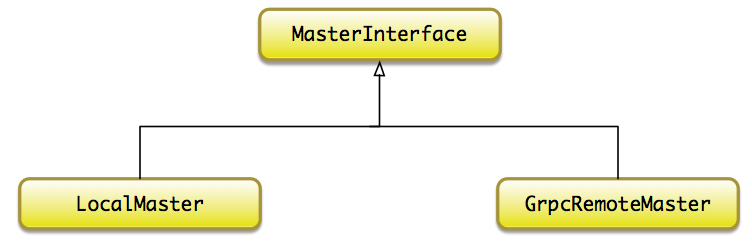
\includegraphics[width=0.6\textwidth]{figures/dist-master-interface.png}
\caption{\code{MasterInterface}}
 \label{fig:dist-master-interface}
\end{figure}

在分布式模式中,\code{GrpcRemoteMaster}使用如下类似的伪代码,并通过\ascii{gRPC}获取远端\code{MasterService}服务。

\begin{leftbar}
\begin{c++}
stub = NewStub("/job:worker/replica:0/task:0")
handle = stub->CreateSession({graph_def})
do {
  stub->RunStep(handle, feeds, fetches);
} while (!should_stop());
stub->CloseSession({handle})
\end{c++}
\end{leftbar}

\subsection{RPC过程}

如\refig{dist-client-master-interaction}所示,\ascii{Client}通过\code{MasterInterface}获取远端\ascii{MasterService}的服务。

\begin{figure}[H]
\centering
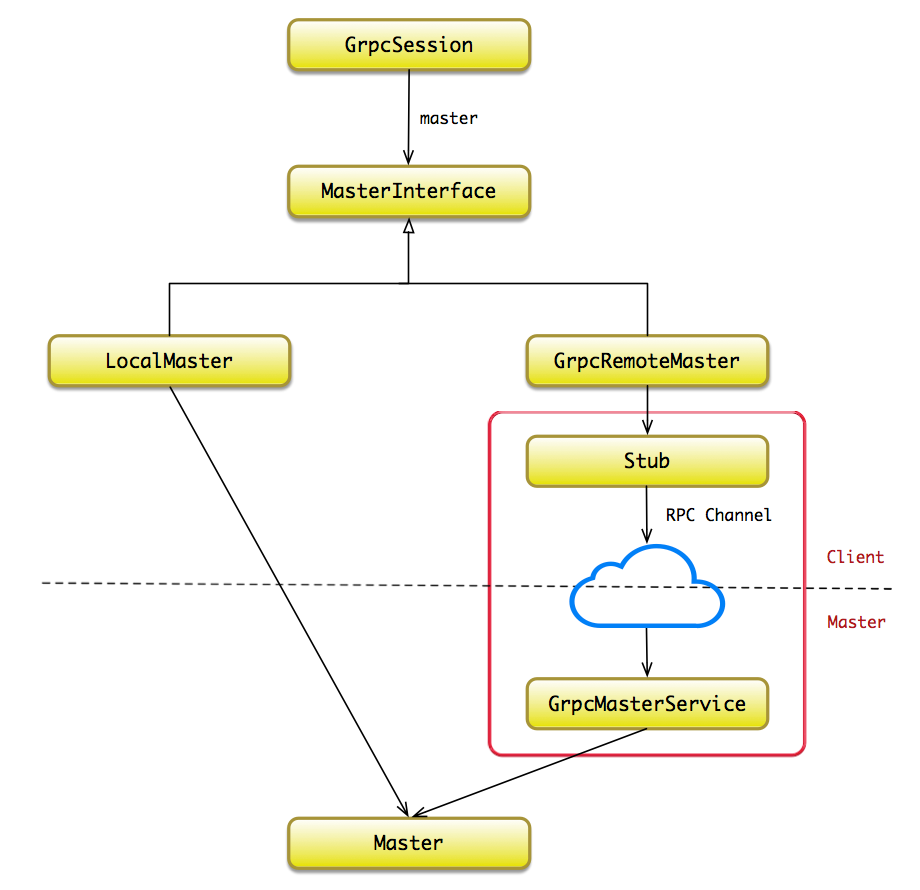
\includegraphics[width=0.8\textwidth]{figures/dist-client-master-interaction.png}
\caption{Client获取MasterService的原理}
 \label{fig:dist-client-master-interaction}
\end{figure}

其中,\code{GrpcRemoteMaster}是\ascii{gRPC}客户端的一种实现,它最终通过\code{Stub}获取远端\ascii{Master}上的\code{GrpcMasterService}服务,使得其行为表现得犹如本地函数调用一般。其中,\code{GrpcMasterService}实现了\code{MasterService}定义的所有服务接口,它是\code{MasterService}真正的服务实体。

\begin{remark}
从严格意义上讲,\script{GrpcSession, ClientMaster, GrpcRemoteMaster}都是\ascii{Client}实现的一部分。而不是通常理解的那样,\ascii{Python}前端系统是完整的\ascii{Client}实现,后端\ascii{C++}后端系统不包括\ascii{Client}的任何实现。
\end{remark}

\subsection{消息定义}

接下来,将详细看看各个接口的消息定义。其中,最重要的就是识别出各个服务的标识。例如,\ascii{Master}可以供多个\ascii{Client}接入,并为每个\ascii{Client}生成对应的\code{MasterSession}实例。因此\code{GrpcSession}持有\code{MasterSession}句柄,实现\ascii{Client}获取\ascii{Master}的服务。

\subsubsection{CreateSession}

如\refig{dist-ms-create-sess-req}所示,\code{CreateSessionRequest}消息中携带初始的计算图,并与\code{target}指定的\ascii{Master}建立连接。当\ascii{Master}收到请求消息后,建立一个相对应的\code{MasterSession}实例,并使用\code{session\_handle}唯一地标识该\code{MasterSession}实例。

待\ascii{Master}逻辑处理完成后,通过返回消息\code{CreateSessionResponse}给\ascii{Client}。其中,\code{CreateSessionResponse}消息中携带\code{session\_handle},通过它\ascii{Client}端的\code{GrpcSession}与\ascii{Master}端的\code{MasterSession}建立关联关系。随后,\ascii{Client}与\ascii{Master}的所有交互中,在请求消息中通过携带\code{session\_handle},\ascii{Master}通过它索引与之相对应的\ascii{MasterSession}实例。

此外,\code{CreateSessionResponse}也携带了初始的\code{graph\_version},用于后续发起\code{ExtendSession}操作,往原始的计算图中追加新的节点。

\begin{figure}[H]
\centering
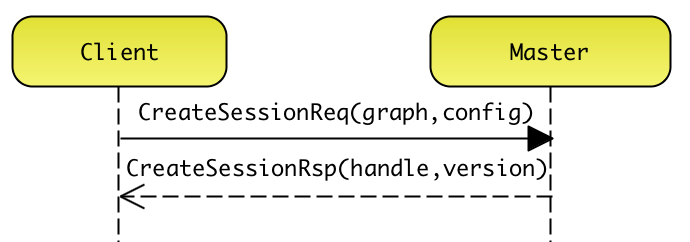
\includegraphics[width=0.6\textwidth]{figures/dist-ms-create-sess-req.png}
\caption{\code{CreateSession}}
 \label{fig:dist-ms-create-sess-req}
\end{figure}

\begin{leftbar}
\begin{c++}
message CreateSessionRequest {
  GraphDef graph_def = 1;
  ConfigProto config = 2;
  string target = 3;
}

message CreateSessionResponse {
  string session_handle = 1;
  int64 graph_version = 2;
}
\end{c++}
\end{leftbar}

\subsubsection{ExtendSession}

当\ascii{CreateSession}成功后,后续\ascii{Client}可以通过\code{ExtendSession},携带待扩展的子图给\ascii{Master},增加原有计算图的规模(只能追加子图,不能修改或删除节点)。

如\refig{dist-ms-extend-sess-req}所示,在请求消息中需要携带\code{current\_graph\_version},\ascii{Master}端进行版本匹配验证;待\code{ExtendSession}的逻辑处理完成后,在响应消息中携带\code{new\_graph\_version},用于下一此\code{ExtendSession}操作。其中,初始的\code{graph\_version}由\code{CreateSessionResponse}携带给\ascii{Client}的。

\begin{figure}[H]
\centering
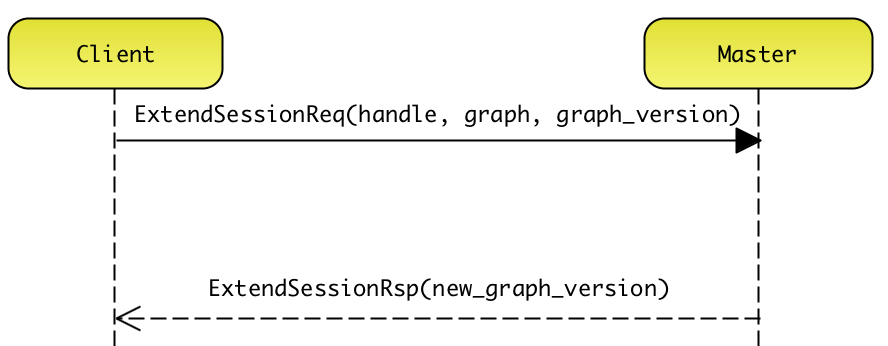
\includegraphics[width=0.7\textwidth]{figures/dist-ms-extend-sess-req.png}
\caption{\code{ExtendSession}}
 \label{fig:dist-ms-extend-sess-req}
\end{figure}

\begin{leftbar}
\begin{c++}
message ExtendSessionRequest {
  string session_handle = 1;

  // REQUIRED: The nodes to be added to the session's graph. 
  // If any node has the same name as an existing node, 
  // the operation will fail with ILLEGAL\_ARGUMENT.
  GraphDef graph_def = 2;

  // REQUIRED: The version number of the graph to be extended. 
  // This will be tested against the current server-side version 
  // number, and the operation will fail with FAILED\_PRECONDITION 
  // if they do not match.
  int64 current_graph_version = 3;
}

message ExtendSessionResponse {
  // The new version number for the extended graph, 
  // to be used in the next call to ExtendSession.
  int64 new_graph_version = 4;
}
\end{c++}
\end{leftbar}

\subsubsection{RunStep}

一般地,在客户端迭代地执行\code{RunStep}。如\refig{dist-ms-run-step-req}所示,在每一次\code{RunStep}执行过程中,\ascii{Client}在请求消息中携带\code{feed, fetch, target},分别表示输入的\ascii{NamedTensor}列表,待输出\ascii{Tensor}的名称列表,待执行\ascii{OP}的名称列表;在响应消息中携带\code{tensor},表示对应于\code{fetch}的名字列表,输出的\ascii{Tensor}列表。

\begin{figure}[H]
\centering
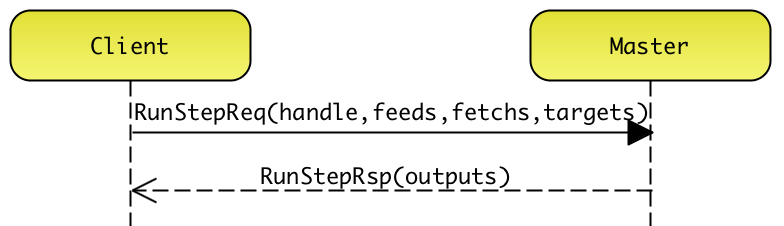
\includegraphics[width=0.7\textwidth]{figures/dist-ms-run-step-req.png}
\caption{\code{RunStep}}
 \label{fig:dist-ms-run-step-req}
\end{figure}

\begin{leftbar}
\begin{c++}
message RunStepRequest {
  string session_handle = 1;

  repeated NamedTensorProto feed = 2;
  repeated string fetch = 3;
  repeated string target = 4;

  RunOptions options = 5;
  string partial_run_handle = 6;
}

message RunStepResponse {
  repeated NamedTensorProto tensor = 1;
  RunMetadata metadata = 2;
}
\end{c++}
\end{leftbar}

\subsubsection{CloseSession}

当计算完成后,需要关闭会话,释放系统计算资源。如\refig{dist-ms-closs-sess}所示,\ascii{Client}通过发送\code{CloseSession}给\ascii{Master},启动计算资源的释放过程。

\begin{figure}[H]
\centering
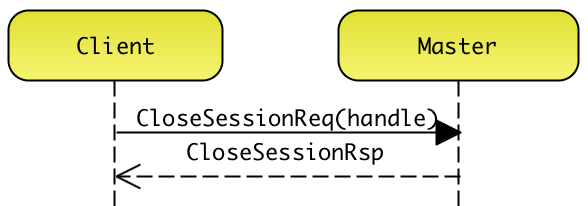
\includegraphics[width=0.5\textwidth]{figures/dist-ms-closs-sess.png}
\caption{\code{CloseSession}}
 \label{fig:dist-ms-closs-sess}
\end{figure}

\begin{leftbar}
\begin{c++}
message CloseSessionRequest {
  string session_handle = 1;
}

message CloseSessionResponse {
}
\end{c++}
\end{leftbar}

\section{Worker服务}

\begin{content}

\code{WorkerService}也是一个\ascii{gRPC}服务,负责调度本地设备集执行本地子图。它定义了接入\ascii{Worker}的接口规范,即\code{master\_service.proto}中定义的接口。

\ascii{Master}根据\code{ClusterSpec}信息,找到集群中其他的\ascii{Server}实例,此时这些\ascii{Server}实例将扮演\ascii{Worker}的角色。\ascii{Master}将子图分发给各个\ascii{Worker}节点,并启动各个\ascii{Worker}节点的子图计算的执行过程。

如果\ascii{Worker}之间存在数据依赖,则通过进程间通信完成交互。其中,\ascii{Master}与\ascii{Worker}之间,\ascii{Worker}与\ascii{Worker}之间的交互遵循\code{WorkerService}定义的接口规范。

\subsection{接口定义}

在\code{worker\_service.proto}文件中,定义了\code{WorkerService}的所有接口;而在\code{worker.proto}文件中,定义了各个接口的消息体。

\begin{leftbar}
\begin{c++}
service WorkerService {
  rpc GetStatus(GetStatusRequest) 
      returns (GetStatusResponse);

  rpc CreateWorkerSession(CreateWorkerSessionRequest)
      returns (CreateWorkerSessionResponse);

  rpc RegisterGraph(RegisterGraphRequest) 
      returns (RegisterGraphResponse);

  rpc DeregisterGraph(DeregisterGraphRequest) 
      returns (DeregisterGraphResponse);

  rpc RunGraph(RunGraphRequest) 
      returns (RunGraphResponse);

  rpc CleanupGraph(CleanupGraphRequest) 
      returns (CleanupGraphResponse);

  rpc CleanupAll(CleanupAllRequest) 
      returns (CleanupAllResponse);

  rpc RecvTensor(RecvTensorRequest) 
      returns (RecvTensorResponse) {
  }

  rpc Logging(LoggingRequest) 
      returns (LoggingResponse);

  rpc Tracing(TracingRequest) 
      returns (TracingResponse);
}
\end{c++}
\end{leftbar}

\subsection{访问服务}

一般地,\ascii{Master/Worker}使用接口\code{WorkerInterface}获取远端\code{WorkerService}的服务。其中,\code{WorkerInterface}定义了异步访问\code{WorkerService}的接口;与\code{MasterInterface}类似,因为\code{RunGraphRequest/RunGraphResponse}中可能含有较大的\code{Tensor},为了避免不必要的对象拷贝,特化了实现了消息的包装器。

\begin{leftbar}
\begin{c++}
struct WorkerInterface {
  // async interfaces.
  virtual void GetStatusAsync(
      const GetStatusRequest* request,
      GetStatusResponse* response,
      StatusCallback done) = 0;

  virtual void CreateWorkerSessionAsync(
      const CreateWorkerSessionRequest* request,
      CreateWorkerSessionResponse* response, 
      StatusCallback done) = 0;

  virtual void RegisterGraphAsync(
      const RegisterGraphRequest* request,
      RegisterGraphResponse* response,
      StatusCallback done) = 0;

  virtual void DeregisterGraphAsync(
      const DeregisterGraphRequest* request,
      DeregisterGraphResponse* response,
      StatusCallback done) = 0;

  virtual void RunGraphAsync(
      CallOptions* opts, 
      RunGraphRequestWrapper* request,
      MutableRunGraphResponseWrapper* repsonse,
      StatusCallback done) = 0;

  // Wrapper classes for the `WorkerService.RunGraph` message.
  //
  // The `RunGraphRequest/RunGraphResponse` message can contain 
  // potentially large tensor data as part of its `send/response`
  // submessages.
  virtual void RunGraphAsync(
      CallOptions* opts, 
      const RunGraphRequest* request,
      RunGraphResponse* response, 
      StatusCallback done) {
    RunGraphRequestWrapper* wrapped_request = 
        new ProtoRunGraphRequest(request);
    MutableRunGraphResponseWrapper* wrapped_response =
        new NonOwnedProtoRunGraphResponse(response);
    RunGraphAsync(opts, wrapped_request, wrapped_response,
        [wrapped_request, wrapped_response, done](const Status& s) {
            done(s);
            delete wrapped_request;
            delete wrapped_response;
        });
  }

  // Returns a request object for use in calls to
  // `RunGraphAsync()`. Ownership is transferred to the caller.
  virtual MutableRunGraphRequestWrapper* CreateRunGraphRequest() {
    return new MutableProtoRunGraphRequest;
  }

  // Returns a response object for use in calls to
  // `RunGraphAsync()`. Ownership is transferred to the caller.
  virtual MutableRunGraphResponseWrapper* CreateRunGraphResponse() {
    return new OwnedProtoRunGraphResponse;
  }

  virtual void CleanupGraphAsync(
      const CleanupGraphRequest* request,
      CleanupGraphResponse* response,
      StatusCallback done) = 0;

  virtual void CleanupAllAsync(
      const CleanupAllRequest* request,
      CleanupAllResponse* response,
      StatusCallback done) = 0;

  virtual void RecvTensorAsync(
      CallOptions* opts,
      const RecvTensorRequest* request,
      TensorResponse* response,
      StatusCallback done) = 0;

  virtual void LoggingAsync(
      const LoggingRequest* request,
      LoggingResponse* response, 
      StatusCallback done) = 0;

  virtual void TracingAsync(
      const TracingRequest* request,
      TracingResponse* response, 
      StatusCallback done) = 0;
};
\end{c++}
\end{leftbar}


\code{WorkerInterface}同时也定义了同步访问接口。同步接口通过\code{CallAndWait}的适配器,间接实现于异步接口之上。特殊地,同步接口使得\ascii{Master/Worker}调用远端\code{WorkerService}具有犹如调用本地函数一般。

\begin{leftbar}
\begin{c++}
struct WorkerInterface {
  // sync interfaces.
  Status GetStatus(
      const GetStatusRequest* request,
      GetStatusResponse* response) {
    return CallAndWait(&ME::GetStatusAsync, request, response);
  }

  Status CreateWorkerSession(
      const CreateWorkerSessionRequest* request,
      CreateWorkerSessionResponse* response) {
    return CallAndWait(&ME::CreateWorkerSessionAsync, request, response);
  }

  Status RegisterGraph(
      const RegisterGraphRequest* request,
      RegisterGraphResponse* response) {
    return CallAndWait(&ME::RegisterGraphAsync, request, response);
  }

  Status DeregisterGraph(
      const DeregisterGraphRequest* request,
      DeregisterGraphResponse* response) {
    return CallAndWait(&ME::DeregisterGraphAsync, request, response);
  }

  Status CleanupGraph(
      const CleanupGraphRequest* request,
      CleanupGraphResponse* response) {
    return CallAndWait(&ME::CleanupGraphAsync, request, response);
  }

  Status CleanupAll(
      const CleanupAllRequest* request,
      CleanupAllResponse* response) {
    return CallAndWait(&ME::CleanupAllAsync, request, response);
  }

  Status Logging(
      const LoggingRequest* request, 
      LoggingResponse* response) {
    return CallAndWait(&ME::LoggingAsync, request, response);
  }

  Status Tracing(
      const TracingRequest* request, 
      TracingResponse* response) {
    return CallAndWait(&ME::TracingAsync, request, response);
  }
 
 private:
  typedef WorkerInterface ME;

  template <typename Method, typename Req, typename Resp>
  Status CallAndWait(Method func, const Req* req, Resp* resp) {
    Status ret;
    Notification n;
    (this->*func)(req, resp, [&ret, &n](const Status& s) {
      ret = s;
      n.Notify();
    });
    n.WaitForNotification();
    return ret;
  }
};
\end{c++}
\end{leftbar}

特殊地,\code{WorkerInterface}生成的实例由\code{WorkerCacheInterface::ReleaseWorker}负责删除。因此,此处为了避免外部非法删除\code{WorkerInterface}实例,限制\code{WorkerInterface}的析构函数为\code{protected},并且声明\code{WorkerCacheInterface}为友元。

\begin{leftbar}
\begin{c++}
struct WorkerInterface {
 protected:
  virtual ~WorkerInterface() {}
  friend class WorkerCacheInterface;
};
\end{c++}
\end{leftbar}

如\refig{dist-worker-interface}所示,\code{WorkerService}存在两种实现。其中,在本地模式中,直接使用\code{GrpcWorker};在分布式模式中,\ascii{Worker}部署在另一个不同的进程内,使用\code{GrpcRemoteWorker}。

\begin{figure}[H]
\centering
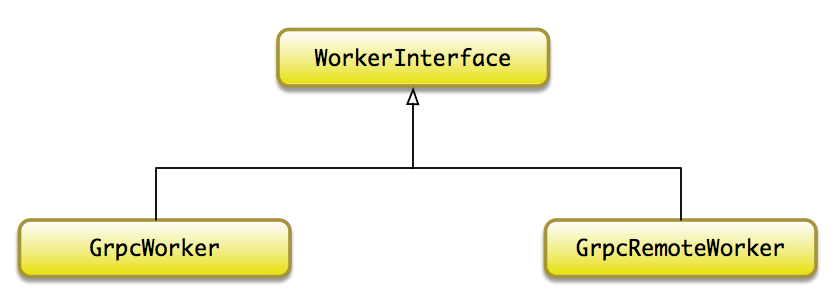
\includegraphics[width=0.6\textwidth]{figures/dist-worker-interface.png}
\caption{\code{WorkerInterface}接口}
 \label{fig:dist-worker-interface}
\end{figure}

\subsection{RPC过程}

如\refig{dist-worker-interaction}所示,在分布式模式中,\code{GrpcRemoteWorker}是\ascii{gRPC}客户端的一种实现,它最终通过\code{Stub}获取远端\ascii{Worker}上的\code{GrpcWorkerService}服务,使得其行为表现得犹如本地函数调用一般。其中,\code{GrpcWorkerService}实现了\code{WorkerService}定义的所有服务接口。

\begin{remark}
从严格意义上讲,\script{GrpcRemoteWorker}是\ascii{Master}或者对端\ascii{Worker}实现的一部分。
\end{remark}

而在本地模式中,通过\code{GrpcWorker}的函数调用,直接获取到了\ascii{WorkerService}的服务,避免了额外的网络传输开销。

\begin{figure}[H]
\centering
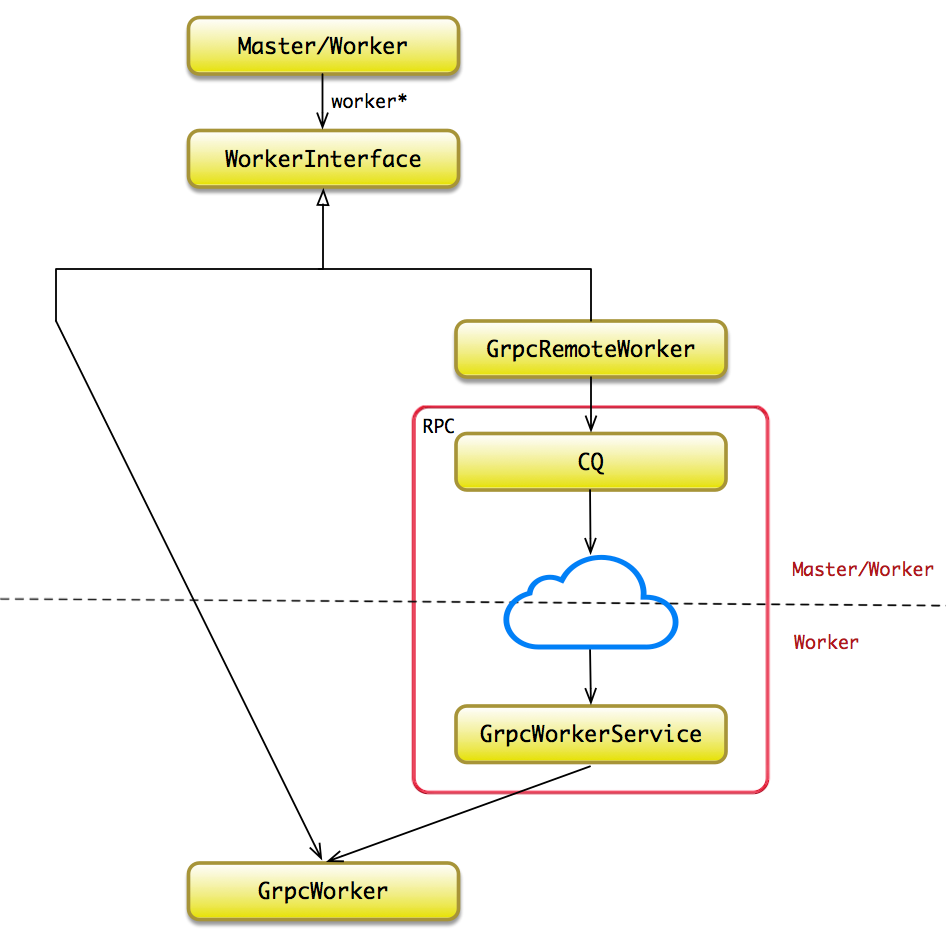
\includegraphics[width=0.7\textwidth]{figures/dist-worker-interaction.png}
\caption{获取\code{MasterService}的RPC过程}
 \label{fig:dist-worker-interaction}
\end{figure}

\subsection{消息定义}

接下来,将详细看看\code{WorkerService}各个接口的消息定义。其中,最重要的就是识别出各个服务的标识。当创建\code{WorkerSession}时,\code{MasterSession}的标识传递给\ascii{Worker},实现了\code{MasterSession}统一管理多个隶属的\code{WorkerSession}实例。

当\code{Worker}首次完成\code{RegisterGraph}后,向\code{Master}返回唯一的\code{graph\_handle},以此标识该图实例。因此,在集群内可以使用\code{(session\_handle, graph\_handle)}二元组唯一标识该图实例。

当\ascii{Master}广播通知各个\ascii{Worker}并发地\code{RunGraph}。为了区分不同\code{step},\ascii{Master}生成全局唯一的\code{step\_id},并通过\code{RunGraph}传递给各个\ascii{Worker}。

\begin{enum}
  \eitem{\code{session\_handle}: 创建\code{MasterSession}实例时自动生成,通过\code{CreateSessionResponse}携带给\ascii{Client};通过\code{CreateWorkerSessionRequest}携带给\ascii{Worker};}  
  \eitem{\code{graph\_id}: 首次\code{RegisterGraph}时由\code{Worker}生成,通过\code{RegisterGraphResponse}携带给\code{Master};}
  \eitem{\code{step\_id}: 每次\code{RunStep}时,由\code{Master}生成唯一的标识,通过\code{RunGraphRequest}携带给\ascii{Worker}。} 
\end{enum}

\subsubsection{CreateWorkerSession}

如\refig{dist-worker-create-worker-sess}所示,\code{CreateWorkerSessionRequest}消息中携带\code{MasterSession}分配的\code{session\_handle}。当\ascii{Worker}收到请求消息后,生成一个\code{WorkerSession}实例,并使用\code{session\_handle}在该\ascii{Worker}内唯一地标识该实例。

在同一个集群中,对于一个\code{MasterSession}实例,其他\ascii{Worker}收到相同的\code{session\_handle}。如此,该\code{MasterSession}实例便能统一管理隶属于它的所有\code{WorkerSession}实例。

\begin{figure}[H]
\centering
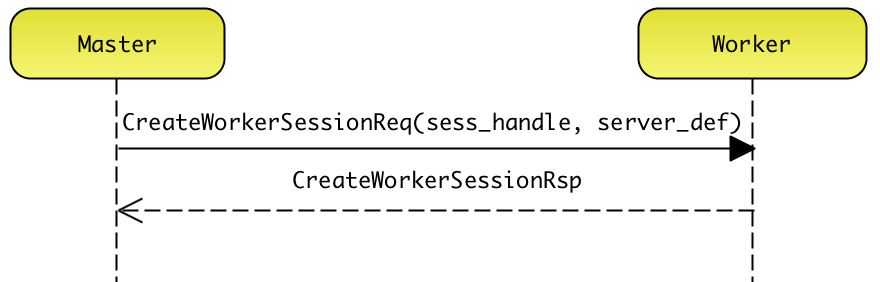
\includegraphics[width=0.6\textwidth]{figures/dist-worker-create-worker-sess.png}
\caption{\code{CreateWorkerSession}}
 \label{fig:dist-worker-create-worker-sess}
\end{figure}

\begin{leftbar}
\begin{c++}
message CreateWorkerSessionRequest {
  string session_handle = 1;
  ServerDef server_def = 2;
}

message CreateWorkerSessionResponse {
}
\end{c++}
\end{leftbar}

\subsubsection{RegisterGraph}

如\refig{dist-worker-register-graph}所示,\code{RegisterGraphRequest}消息中携带\code{MasterSession}分配的\code{session\_handle},及其子图实例\ascii{graph\_def}。当\code{Worker}完成子图注册及其初始化后,向\ascii{Master}返回该子图的\code{graph\_handle}。

需要注意的是,\code{Master}只会在执行一次\code{RegisterGraph},除非计算图的节点被重新编排,或者\code{Master}进程被重启。

\begin{figure}[H]
\centering
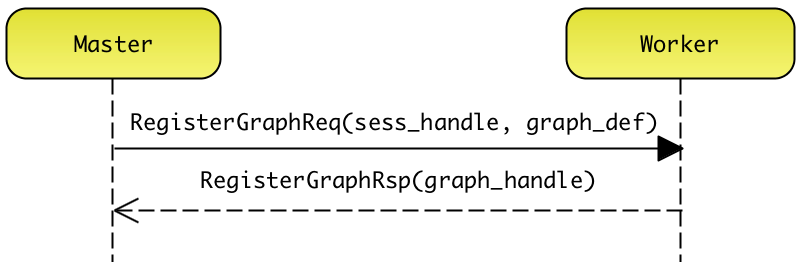
\includegraphics[width=0.6\textwidth]{figures/dist-worker-register-graph.png}
\caption{\code{RegisterGraph}}
 \label{fig:dist-worker-register-graph}
\end{figure}

\begin{leftbar}
\begin{c++}
message RegisterGraphRequest {
  string session_handle = 1;

  GraphDef graph_def = 2;
  bool has_control_flow = 3 [deprecated = true];

  GraphOptions graph_options = 4;
  DebugOptions debug_options = 5;
}

message RegisterGraphResponse {
  string graph_handle = 1;
}
\end{c++}
\end{leftbar}


\subsubsection{DeregisterGraph}

如\refig{dist-worker-deregister-graph}所示,当\code{Worker}节点上的子图不再需要时(例如,计算图被重新调度,图中节点被重新编排),此时\code{Master}向\ascii{Worker}发送\code{DeregisterGraph}消息,以便\code{Worker}注销掉该子图实例。

\begin{figure}[H]
\centering
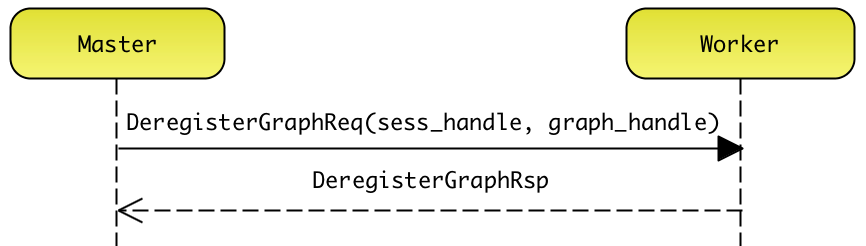
\includegraphics[width=0.6\textwidth]{figures/dist-worker-deregister-graph.png}
\caption{\code{DeregisterGraph}}
 \label{fig:dist-worker-deregister-graph}
\end{figure}

\begin{leftbar}
\begin{c++}
message DeregisterGraphRequest {
  string session_handle = 2;
  string graph_handle = 1;
}

message DeregisterGraphResponse {
}
\end{c++}
\end{leftbar}

\subsubsection{RunGraph}

执行\ascii{Worker}节点上注册的子图时,为了区分不同\code{step},\ascii{Master}生成唯一\code{step\_id}并传递给各个\ascii{Worker},各个\ascii{Worker}通过\code{step\_id}实现数据的协同。

此外,\code{RunGraphRequest}携带了\code{send, recv\_key},分别表示子图输入的\code{Tensor}标识和数据,及其子图输出的\code{Tensor}的标识。\code{RunGraphResponse}返回\code{recv\_key}相对应的\code{Tensor}列表。

\begin{figure}[H]
\centering
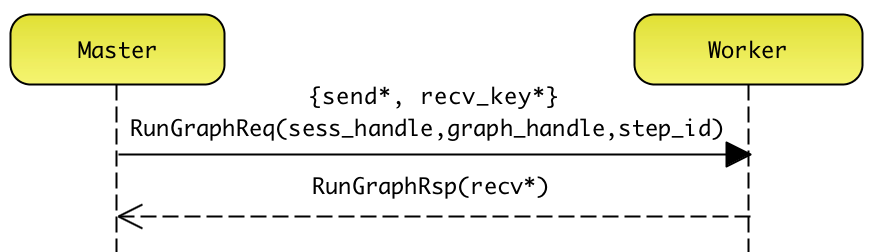
\includegraphics[width=0.6\textwidth]{figures/dist-worker-run-graph.png}
\caption{\code{RunGraph}}
 \label{fig:dist-worker-run-graph}
\end{figure}

\begin{leftbar}
\begin{c++}
message RunGraphRequest {
  string session_handle = 8;
  string graph_handle = 1;
  int64 step_id = 2;

  ExecutorOpts exec_opts = 5;

  repeated NamedTensorProto send = 3;
  repeated string recv_key = 4;

  bool is_partial = 6;
  bool is_last_partial_run = 7;
}

message RunGraphResponse {
  repeated NamedTensorProto recv = 1;

  // execution stats
  StepStats step_stats = 2;
  CostGraphDef cost_graph = 3;
  repeated GraphDef partition_graph = 4;
}
\end{c++}
\end{leftbar}

\subsubsection{RecvTensor}

当执行某一次\code{step}中,如果两个\ascii{Worker}需要交互数据,消费者向生产者发送\code{RecvTensorRequest}消息,通过携带\code{(step\_id, rendezvous\_key)}二元组,请求对端\ascii{Worker}相应的\code{Tensor}数据,并通过\code{RecvTensorResponse}返回。

\begin{figure}[H]
\centering
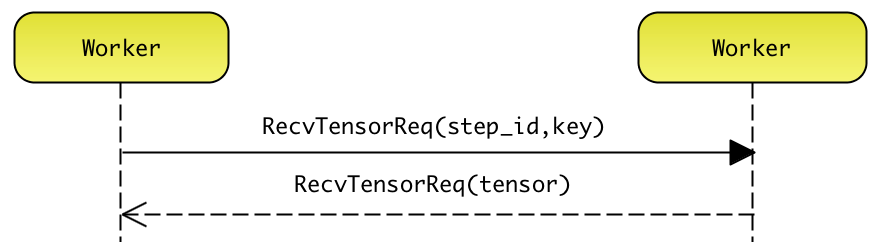
\includegraphics[width=0.6\textwidth]{figures/dist-worker-recv-tensor.png}
\caption{\code{RecvTensor}}
 \label{fig:dist-worker-recv-tensor}
\end{figure}

\begin{leftbar}
\begin{c++}
message RecvTensorRequest {
  int64 step_id = 1;
  string rendezvous_key = 2;

  // If true, use an out-of-band DMA mechanism to transfer the
  // received tensor.
  bool dma_ok = 3;

  // Optional information on client-side device locality.
  DeviceLocality client_locality = 4;

  // Optional information on server-side device locality.
  DeviceLocality server_locality = 5;

  // Optional information needed by the RPC subsystem.
  google.protobuf.Any transport_options = 6;
}

message RecvTensorResponse {
  // The tensor as a proto.
  TensorProto tensor = 1;

  // If true, this tensor was the output of a dead node, and the
  // content is invalid.
  bool is_dead = 2;

  // The time at which tensor was available and started to be returned.
  int64 send_start_micros = 3;

  // Optional additional information about how to receive the tensor,
  // e.g. in the event that `RecvTensorRequest.dma\_ok` was true.
  google.protobuf.Any transport_options = 4;
}
\end{c++}
\end{leftbar}

\end{content}

\section{会话控制}

\emph{会话控制}是\tf{}分布式运行时的核心,也是整个\tf{}执行引擎的的关键路径。为了理顺会话控制的脉络,接下来的文章将重点讲述整个会话控制的详细过程。

\begin{content}

\subsection{会话协同}

如\refig{dist-session-overview}所示,在分布式模式中,会话控制通过\code{GrpcSession, MasterSession, WorkerSession}之间的协同实现的,它们分别驻留在\code{Client, Master, Worker}上,使用同一个\code{session\_handle}实现协同工作的。

其中,\code{tf.Session}使用\ascii{Python}实现,是\tf{}对外提供的\ascii{API}。它与\code{GrpcSession}在同一个进程内,并且直接持有\code{GrpcSession}的句柄(或指针)实现的。

\begin{figure}[H]
\centering
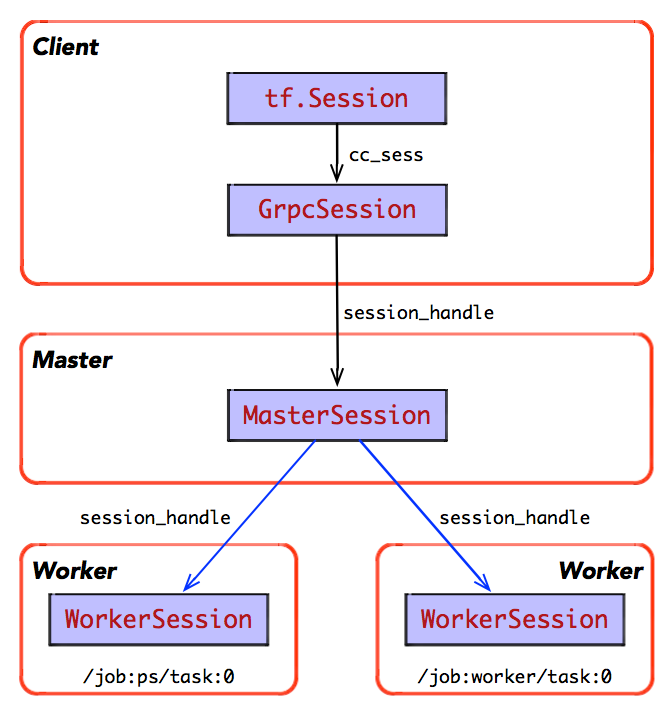
\includegraphics[width=0.6\textwidth]{figures/dist-session-overview-1.png}
\caption{会话协同}
 \label{fig:dist-session-overview}
\end{figure}

如\refig{dist-multi-client-conn}所示,在分布式模式中,可能存在多个\ascii{Client}同时接入一个\ascii{Master},\ascii{Master}为其每个接入的\ascii{Client}创建一个\code{MasterSession}实例。\ascii{Worker}也可能同时为多个\ascii{Master}提供计算服务,\ascii{Worker}为其每个请求计算的\ascii{Master}创建一个\code{WorkerSession}实例。为了区分不同的\ascii{Client}的计算服务,使用不同的\code{session\_handle}区分。

\begin{figure}[H]
\centering
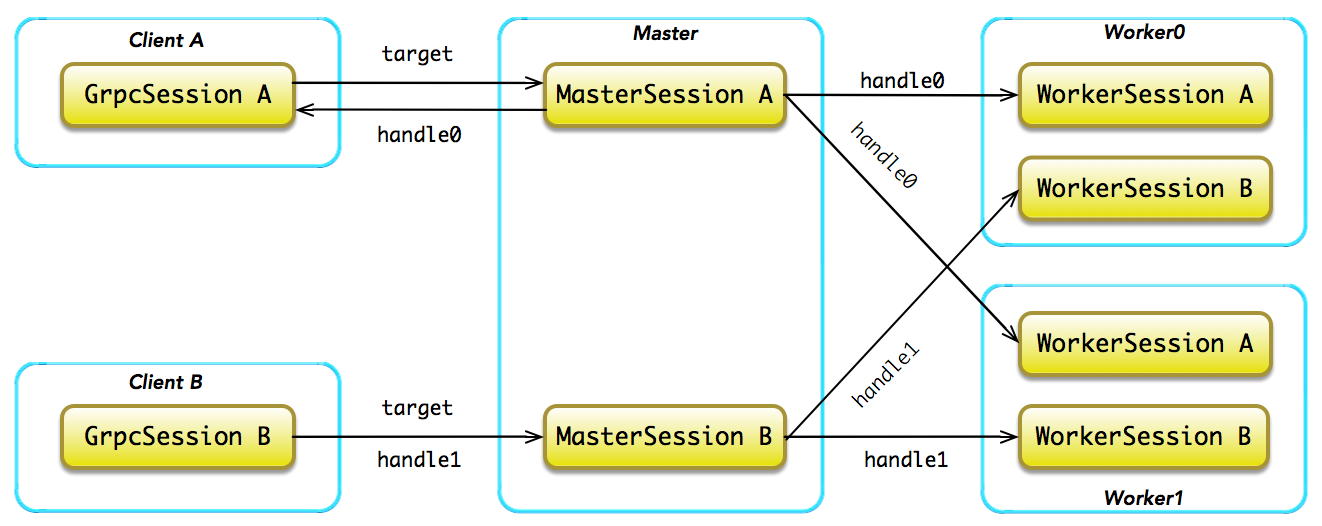
\includegraphics[width=0.9\textwidth]{figures/dist-multi-client-conn.png}
\caption{会话控制:领域模型}
 \label{fig:dist-multi-client-conn}
\end{figure}

\subsection{生命周期}

\code{GrpcSession}控制\ascii{Client}的会话生命周期,\code{MasterSession}控制\ascii{Master}的会话生命周期,\code{WorkerSession}控制\ascii{Worker}的会话生命周期,它们之间通过\code{session\_handle}实现协同。

\subsubsection{GrpcSession生命周期}

在分布式模式下,\code{Client}的运行时由\code{GrpcSession}控制,\code{GrpcSession}的生命周期过程如\refig{dist-grpc-session-life-cycle}所示。

\begin{figure}[H]
\centering
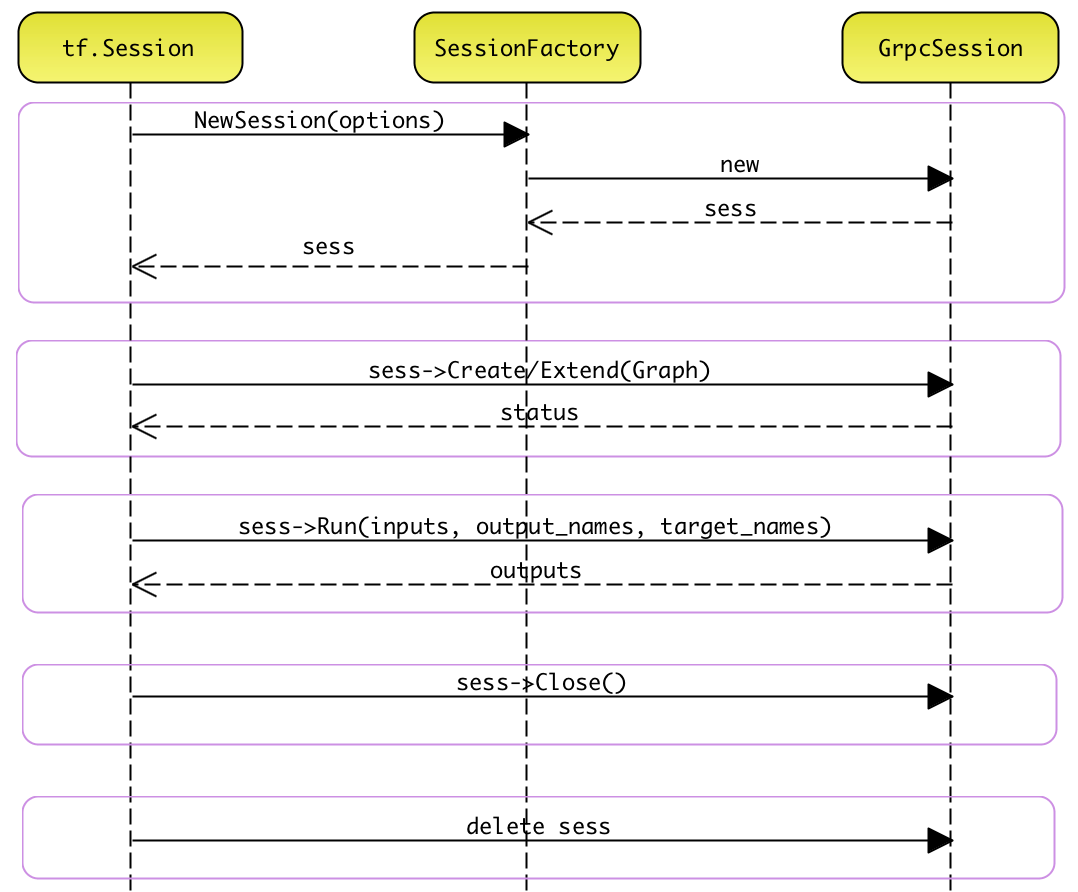
\includegraphics[width=0.8\textwidth]{figures/dist-grpc-session-life-cycle.png}
\caption{\code{GrpcSession}生命周期}
 \label{fig:dist-grpc-session-life-cycle}
\end{figure}

\subsubsection{MasterSession生命周期}

在分布式模式下,\code{Master}的运行时由\code{MasterSession}控制,\code{MasterSession}生命周期过程如\refig{dist-master-session-life-cycle}所示。

\begin{figure}[H]
\centering
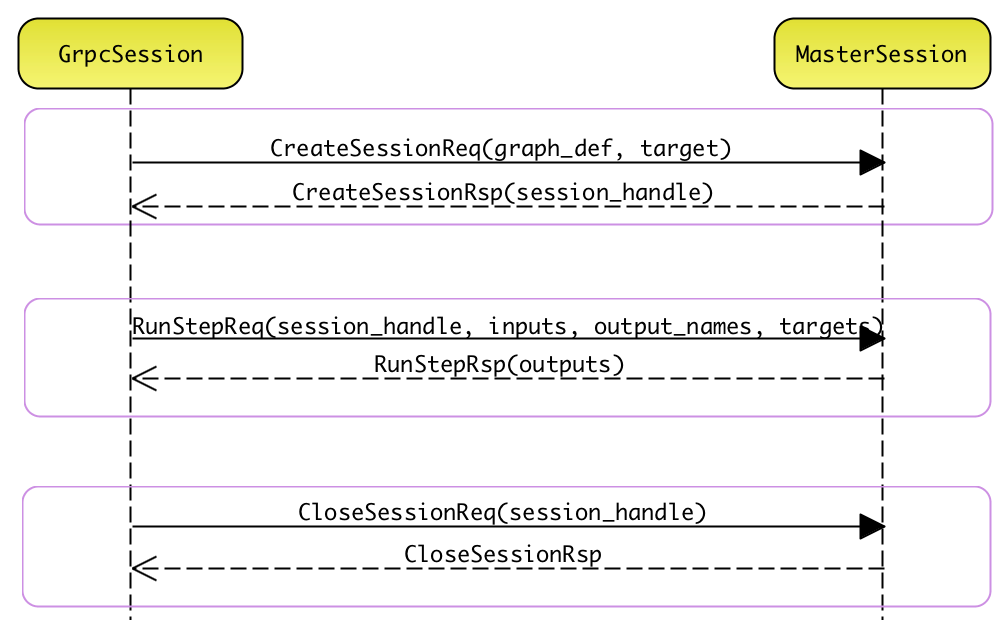
\includegraphics[width=0.8\textwidth]{figures/dist-master-session-life-cycle.png}
\caption{\code{MasterSession}生命周期}
 \label{fig:dist-master-session-life-cycle}
\end{figure}

\subsubsection{WorkerSession生命周期}

在分布式模式下,\code{Worker}的运行时由\code{WorkerSession}控制,\code{WorkerSession}生命周期过程如\refig{dist-worker-session-life-cycle}所示。

\begin{figure}[H]
\centering
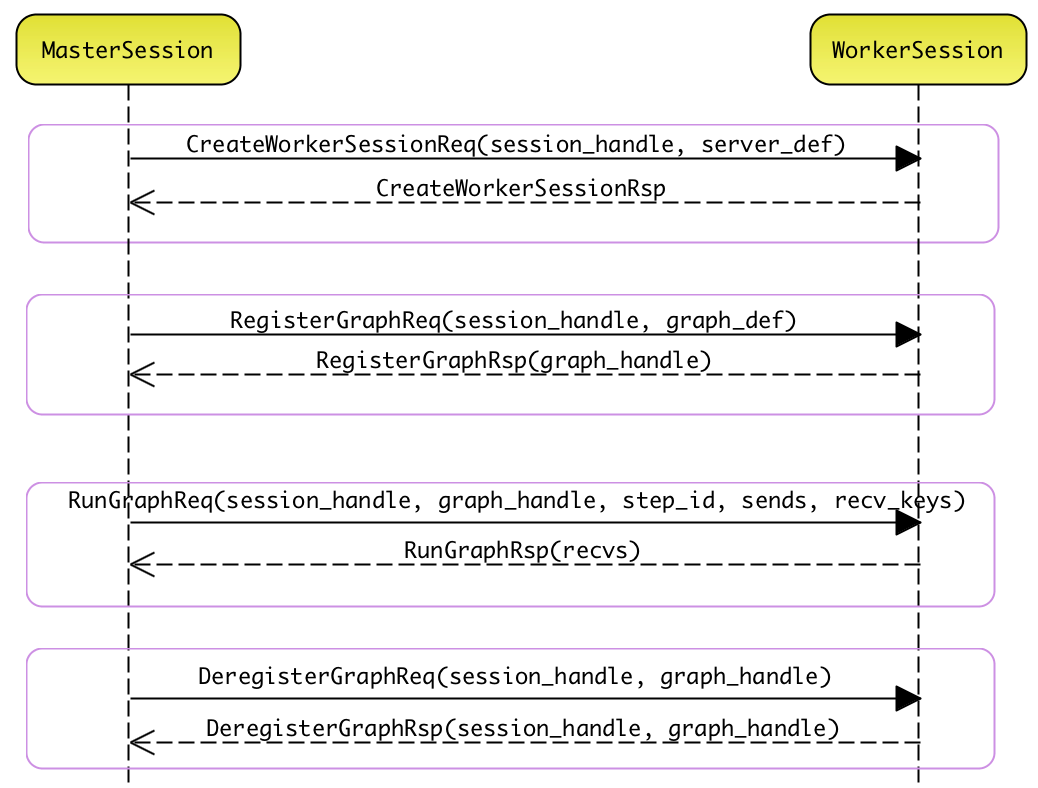
\includegraphics[width=0.8\textwidth]{figures/dist-worker-session-life-cycle.png}
\caption{\code{WorkerSession}生命周期}
 \label{fig:dist-worker-session-life-cycle}
\end{figure}

\subsection{会话过程}

在用户编程环境中,\ascii{Client}从\code{tf.Session(target)}为起点,通过\code{Session.run}启动迭代执行,最终计算完成后调用\code{Session.close}关闭会话。但是,在分布式执行引擎的实现中,其过程要复杂得多。

\begin{nitemize}
  \eitem{创建会话}    
    \begin{enum}
      \eitem{创建\code{GrpcSession};}  
      \eitem{获取远端设备集;} 
      \eitem{创建\code{MasterSession};}
      \eitem{创建\code{WorkerSession};}      
    \end{enum}
  \eitem{迭代执行}          
    \begin{enum}
      \eitem{启动执行;}  
      \eitem{图剪枝;}  
      \eitem{图分裂;}        
      \eitem{注册子图;}              
      \eitem{运行子图;}                         
    \end{enum}      
  \eitem{关闭会话}          
    \begin{enum}          
      \eitem{关闭\code{GrpcSession};}  
      \eitem{关闭\code{MasterSession};}
      \eitem{关闭\code{WorkerSession};}      
    \end{enum}  
\end{nitemize}

\end{content}

\section{创建会话}

\subsection{创建GrpcSession}

\begin{content}

如\refig{dist-grpc-session-factory}所示,\code{GrpcSession}由\code{GrpcSessionFactory}多态创建。

\begin{figure}[H]
\centering
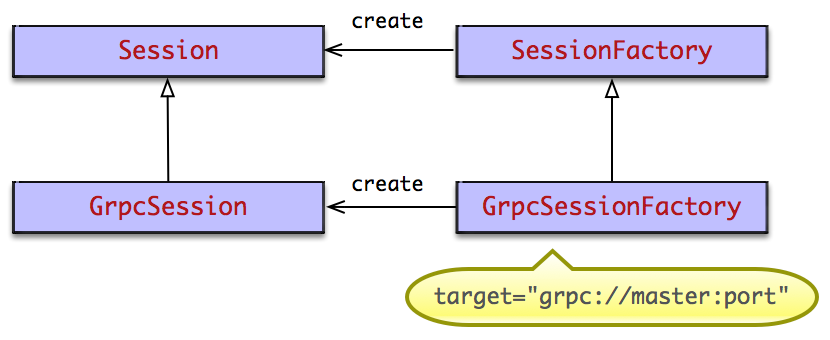
\includegraphics[width=0.6\textwidth]{figures/dist-grpc-session-factory.png}
\caption{多态创建GrpcSession}
 \label{fig:dist-grpc-session-factory}
\end{figure}

\begin{leftbar}
\begin{c++}
const char* kSchemePrefix = "grpc://";

struct GrpcSessionFactory : SessionFactory {
  bool AcceptsOptions(const SessionOptions& options) override {
    return StringPiece(options.target).starts_with(kSchemePrefix);
  }

  Session* NewSession(const SessionOptions& options) override {
    std::unique_ptr<GrpcSession> ret;
    Status s = GrpcSession::Create(options, &ret);
    if (s.ok()) {
      return ret.release();
    } else {
      return nullptr;
    }
  }
};
\end{c++}
\end{leftbar}

当\code{target}以\code{grpc://}开头,则\code{SessionFactory::GetFactory}返回\code{GrpcSessionFactory}实例,而\code{GrpcSessionFactory}工厂方法委托\code{GrpcSession::Create}的静态工厂方法负责创建\code{GrpcSession}实例。

而\code{GrpcSessionFactory::NewSession}由\ascii{C API}调用。其中,\ascii{C API}是\tf{}后端系统对外提供的标准接口,对外供多种编程语言调用。

\begin{leftbar}
\begin{c++}
Status NewSession(const SessionOptions& options, Session** out_session) {
  SessionFactory* factory;
  Status s = SessionFactory::GetFactory(options, &factory);
  if (!s.ok()) {
    *out_session = nullptr;
    return s;
  }
  *out_session = factory->NewSession(options);
  if (!*out_session) {
    return errors::Internal("Failed to create session.");
  }
  return Status::OK();
}

TF_DeprecatedSession* TF_NewDeprecatedSession(
  const TF_SessionOptions* opt, TF_Status* status) {
  Session* session;
  status->status = NewSession(opt->options, &session);
  if (status->status.ok()) {
    return new TF_DeprecatedSession({session});
  } else {
    return nullptr;
  }
}
\end{c++}
\end{leftbar}

在\code{GrpcSession::Create}静态工厂方法中,它主要负责创建\code{GrpcSession}实例,并完成相应的初始化工作。在初始化过程中,最重要的就是构建\code{MasterInterface}实例。其中,\code{MasterInterface}存在两种子类实现,分别对应两种不同应用场景:

\begin{enum}
  \eitem{\code{LocalMaster}:\ascii{Client}与\ascii{Master}在同一进程内,调用\code{LocalMaster::Lookup}直接获取\code{LocalMaster}实例;}
  \eitem{\code{GrpcRemoteMaster}:\ascii{Client}与\ascii{Master}不在同一进程内,调用工厂方法\code{NewGrpcMaster}生成\code{GrpcRemoteMaster}实例。}
\end{enum}

\begin{leftbar}
\begin{c++}
Status GrpcSession::Create(
    const SessionOptions& options,
    std::unique_ptr<GrpcSession>* out_session) {
  std::unique_ptr<GrpcSession> session(new GrpcSession(options));
  std::unique_ptr<MasterInterface> master;
  // intra-process between client and master.
  if (!options.config.rpc_options().use_rpc_for_inprocess_master()) {
    master = LocalMaster::Lookup(options.target);
  }
  // inter-process between client and master.
  if (!master) {
    SharedGrpcChannelPtr master_channel;
    TF_RETURN_IF_ERROR(NewHostPortGrpcChannel(
        options.target.substr(strlen(kSchemePrefix)), &master_channel));
    master.reset(NewGrpcMaster(master_channel));
  }
  session->SetRemoteMaster(std::move(master));
  *out_session = std::move(session);
  return Status::OK();
}
\end{c++}
\end{leftbar}

\end{content}

\subsection{创建MasterSession}

\begin{content}

如\refig{dist-create-master-session}所示,当调用\code{GprcSession::Create}时,将初始的计算图通过\code{CreateSessionRequst}消息发送给\ascii{Master}。

当\ascii{Master}收到\code{CreateSessionRequst}消息后,生成相对应的\code{MasterSession}实例,并使用全局唯一的\code{handle}标识,最终通过\code{CreateSessionResponse}消息带回给\code{GrpcSession}。

\begin{figure}[H]
\centering
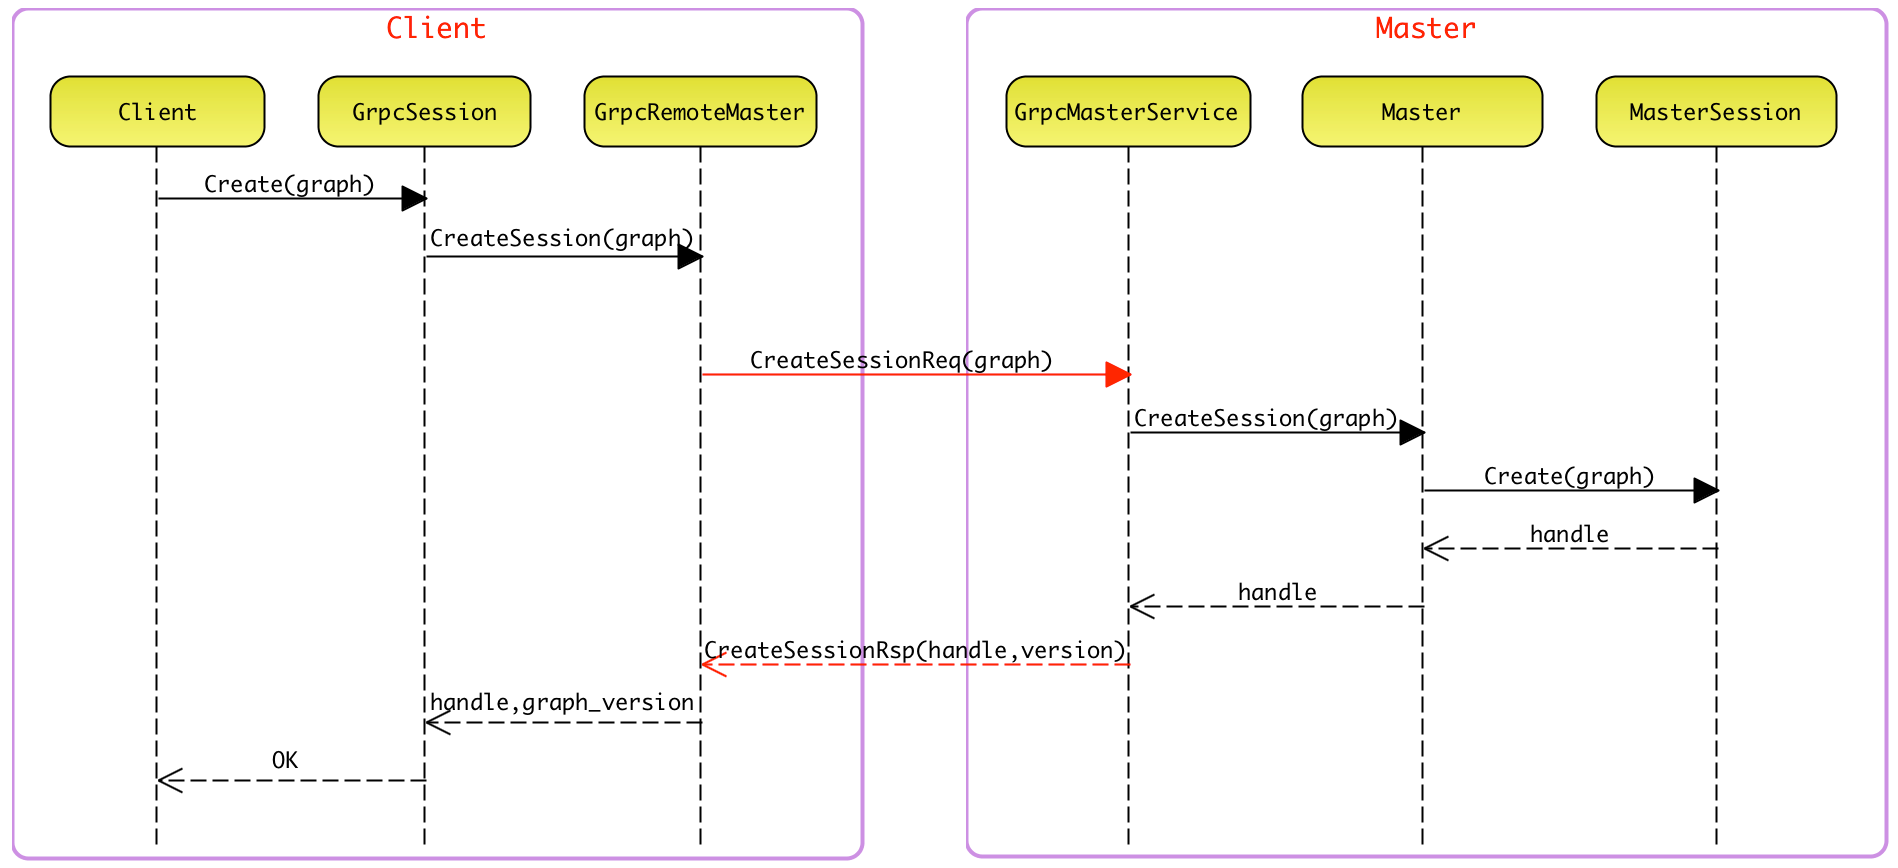
\includegraphics[width=1.0\textwidth]{figures/dist-create-master-session.png}
\caption{创建\code{MasterSession}}
 \label{fig:dist-create-master-session}
\end{figure}

\subsubsection{GrpcSesion::Create(graph\_def)}

\code{GrpcSession::Create(graph\_def)}方法主要用于\code{Client}请求\code{Master}创建\code{MasterSession}实例。首先,\code{GrpcSession::Create}方法完成构造\code{CreateSessionRequst}消息,然后通过\code{GrpcRemoteMaster}将其发送给\ascii{Master}。

接着,等\code{GrpcSession}收到\code{CreateSessionResponse}消息后,保存\code{MasterSession}的\code{handle},及其新的计算图版本号\code{graph\_version}。其中,\code{handle}用于标识\ascii{Master}侧的\code{MasterSession}实例,\code{graph\_version}用于后续扩展计算图使用。

\begin{leftbar}
\begin{c++}
void GrpcSession::BuildCreateSessionReq(
    const GraphDef& graph,
    CreateSessionRequest& req) {
  *req.mutable_config() = options_.config;
  *req.mutable_graph_def() = graph;
  req.set_target(options_.target);
}

void GrpcSession::SaveCreateSessionRsp(
    CreateSessionResponse& rsp) {
  mutex_lock l(mu_);
  swap(handle_, *(resp.mutable_session_handle()));
  current_graph_version_ = resp.graph_version();
}

Status GrpcSession::CreateImpl(CallOptions* call_options,
                               const GraphDef& graph) {
  CreateSessionRequest req;
  CreateSessionResponse resp;

  BuildCreateSessionReq(graph, req);
  Status s = master_->CreateSession(call_options, &req, &resp);
  if (s.ok()) {
    SaveCreateSessionRsp(resp);
  }
  return s;
}

Status GrpcSession::Create(const RunOptions& run_options,
                           const GraphDef& graph) {
  CallOptions call_options;
  call_options.SetTimeout(run_options.timeout_in_ms());
  return CreateImpl(&call_options, graph);
}

Status GrpcSession::Create(const GraphDef& graph) {
  CallOptions call_options;
  call_options.SetTimeout(options_.config.operation_timeout_in_ms());
  return CreateImpl(&call_options, graph);
}
\end{c++}
\end{leftbar}

\subsubsection{GrpcRemoteMaster::CreateSession}

\code{GrpcRemoteMaster}是一个\ascii{gRPC}的客户端实现。它的实现非常简单,通过\ascii{gRPC}的一个\code{stub}调用远端\ascii{Master}相应的服务。

\begin{leftbar}
\begin{c++}
namespace {
  void SetClientContext(
      const CallOptions& call_options,
      ::grpc::ClientContext& ctx) {
    ctx.set_fail_fast(false);
    SetDeadline(&ctx, call_options.GetTimeout());
  }
}

Status GrpcRemoteMaster::CreateSession(
    CallOptions* call_options,
    const CreateSessionRequest* request,
    CreateSessionResponse* response) override {
  ::grpc::ClientContext ctx;
  SetClientContext(*call_options, ctx);
  return FromGrpcStatus(stub_->CreateSession(&ctx, *request, response));
}
\end{c++}
\end{leftbar}

\subsubsection{GrpcMasterService::CreateSessionHandler}

\code{GrpcMasterService}是一个\ascii{gRPC}服务,它实现了\code{MasterService}的\ascii{RPC}服务接口。

当收到\code{CreateSession}消息后,将由\code{GrpcMasterService::CreateSessionHandler}处理该消息。它将委托\code{Master}处理该消息。

\code{Master}处理完成后,将回调完成时的\ascii{lambda}表达式,向\ascii{Client}返回\code{CreateSessionResponse}的响应消息。

\begin{leftbar}
\begin{c++}
// RPC handler for creating a session.
void GrpcMasterService::CreateSessionHandler(
  MasterCall<CreateSessionRequest, CreateSessionResponse>* call) {
  master_impl_->CreateSession(
    &call->request, &call->response,
    [call](const Status& status) {
        call->SendResponse(ToGrpcStatus(status));
    });
  ENQUEUE_REQUEST(CreateSession, true);
}
\end{c++}
\end{leftbar}

\subsubsection{Master::CreateSession}

然后,\code{Master::CreateSession}将会在线程池里启动一个线程,并在线程内按照\code{cluster\_spec}信息,寻找所有的\ascii{Worker},并收集本地设备,及其远端设备的信息。最后,该线程创建了一个\code{MasterSession};并且当创建成功后,\ascii{Master}会保存\code{(handle, master\_session)}的二元组信息,以便后续\ascii{Master}能够通过\code{handle}索引相应的\code{MasterSession}实例。

\begin{leftbar}
\begin{c++}
using RemoveDevices = unique_ptr<vector<unique_ptr<Device>>>;

void Master::CreateSession(const CreateSessionRequest* req,
                           CreateSessionResponse* resp, MyClosure done) {
  SchedClosure([this, req, resp, done]() {
    // 1. Find all workers.  
    // ignore implements...
    std::unique_ptr<WorkerCacheInterface> worker_cache_ptr;

    // 2. Find all remote devices. 
    // ignore implements...
    RemoveDevices remote_devices(new vector<unique_ptr<Device>>());

    // 3. Construct DeviceSet.
    // ignore implements...
    std::unique_ptr<DeviceSet> device_set;

    // 4. Create MasterSession
    SessionOptions options;
    options.config = req->config();
    
    MasterSession* session = env_->master_session_factory(
        options, env_, std::move(remote_devices), 
        std::move(worker_cache_ptr), std::move(device_set));

    GraphDef* gdef =
        const_cast<CreateSessionRequest*>(req)->mutable_graph_def();
    
    // 5. Create WorkerSession foreach worker.
    status = session->Create(gdef, worker_cache_factory_options);
    resp->set_session_handle(session->handle());
    
    // 6. Store <handle, master\_session> pair.
    {
      mutex_lock l(mu_);
      CHECK(sessions_.insert({session->handle(), session}).second);
    }
  });
}
\end{c++}
\end{leftbar}

其中,在创建完\code{MasterSession},并保存\code{(handle, master\_session)}的二元组信息之间,将启动\code{MasterSession::Create(graph\_def)}过程。

\subsubsection{MasterSession::Create(graph\_def)}

\code{MasterSession::Create(graph\_def)}主要完成两件事情。

\begin{enum}
  \eitem{初始化计算图,并生成\code{SimpleGraphExecutionState}实例;}
  \eitem{广播所有\ascii{Worker}创建相应的\code{WorkerSession}实例。}
\end{enum}

\begin{leftbar}
\begin{c++}
Status MasterSession::Create(
    GraphDef* graph_def,
    const WorkerCacheFactoryOptions& options) {
  SimpleGraphExecutionStateOptions execution_options;
  execution_options.device_set = devices_.get();
  execution_options.session_options = &session_opts_;
  {
    mutex_lock l(mu_);
    TF_RETURN_IF_ERROR(SimpleGraphExecutionState::MakeForBaseGraph(
        graph_def, execution_options, &execution_state_));
  }
  if (options.cluster_def != nullptr) {
    return CreateWorkerSessions(options);
  }
  return Status::OK();
}
\end{c++}
\end{leftbar}

\subsection{创建\code{WorkerSession}}

\ascii{Master}会广播所有\ascii{Worker}创建相应的\code{WorkerSession}实例。这些\code{WorkerSession}隶属于此\code{MasterSession}实例,因为它们使用与\code{MasterSession}实例相同的\code{handle}标识。

\code{MasterSession}为了收齐所有\ascii{Worker}返回的\code{CreateWorkerSessionResponse}消息,引入了\code{BlockingCounter}计数器。

\begin{leftbar}
\begin{c++}
struct MasterSession::Worker {
  Worker(MasterSession* sess, const string& name,
         const DeviceNameUtils::ParsedName& parsed_name,
         const WorkerCacheFactoryOptions& opts)
      : sess(sess),
        name(&name),
        worker(GetOrCreateWorker()) {
    BuildRequest(parsed_name, opts);
  }

  void CreateWorkerSession(BlockingCounter& done, Status& status) {
    auto cb = [&status, &done](const Status& s) {
      status.Update(s);
      done.DecrementCount();
    };
    worker->CreateWorkerSessionAsync(&request, &response, cb);
  }

  void Release() {
    if (worker != nullptr) {
      sess->worker_cache_->ReleaseWorker(*name, worker);
    }
  }

 private:
  WorkerInterface* GetOrCreateWorker() {
    return sess->worker_cache_->CreateWorker(*name);
  }

  void BuildRequest(const DeviceNameUtils::ParsedName& parsed_name,
                    const WorkerCacheFactoryOptions& opts) {
    request.set_session_handle(sess->handle_);
    BuildServerDef(parsed_name, opts, request.mutable_server_def());
  }

  void BuildServerDef(const DeviceNameUtils::ParsedName& parsed_name,
                      const WorkerCacheFactoryOptions& opts,
                      ServerDef* server_def) {
    *server_def->mutable_cluster() = *opts.cluster_def;
    server_def->set_protocol(*opts.protocol);
    server_def->set_job_name(parsed_name.job);
    server_def->set_task_index(parsed_name.task);
  }

 private:
  MasterSession* sess;

  // The worker name. (Not owned.)
  const string* name;

  // The worker referenced by name. (Not owned.)
  WorkerInterface* worker = nullptr;

  // Request and responses used for a given worker.
  CreateWorkerSessionRequest request;
  CreateWorkerSessionResponse response;
};

struct MasterSession::WorkerGroup {
  WorkerGroup(MasterSession* sess)
      : sess(sess) {
  }

  Status CreateWorkerSessions(const WorkerCacheFactoryOptions& opts) {
    TF_RETURN_IF_ERROR(CreateWorkers(opts));
    TF_RETURN_IF_ERROR(BroadcastWorkers());
    return Status::OK();
  }

  void ReleaseWorkers() {
    for (auto& worker : workers) {
      worker.Release();
    }
  }

 private:
  Status CreateWorkers(const WorkerCacheFactoryOptions& opts) {
    sess->worker_cache_->ListWorkers(&worker_names);
    for (size_t i = 0; i < worker_names.size(); ++i) {
      TF_RETURN_IF_ERROR(AppendWorker(worker_names[i], opts));
    }
    return Status::OK();
  }

  Status BroadcastWorkers() {
    Status status = Status::OK();
    BlockingCounter done(workers.size());
    for (size_t i = 0; i < workers.size(); ++i) {
      workers[i].CreateWorkerSession(done, status);
    }
    done.Wait();
    return status;
  }

  Status AppendWorker(const string& worker_name,
                    const WorkerCacheFactoryOptions& opts) {
    DeviceNameUtils::ParsedName parsed_name;
    TF_RETURN_IF_ERROR(ParseWorkerName(worker_name, &parsed_name));
    workers.emplace_back(Worker(sess, worker_name, parsed_name, opts));
    return Status::OK();
  }

  Status ParseWorkerName(const string& worker_name,
                         DeviceNameUtils::ParsedName* parsed_name) {
    if (!DeviceNameUtils::ParseFullName(worker_name, parsed_name)) {
      return errors::Internal("Could not parse name ", worker_name);
    }
    if (!parsed_name->has_job || !parsed_name->has_task) {
      return errors::Internal("Incomplete worker name ", worker_name);
    }
    return Status::OK();
  }

 private:
  MasterSession* sess;
  std::vector<string> worker_names;
  std::vector<Worker> workers;
};

Status MasterSession::CreateWorkerSessions(
    const WorkerCacheFactoryOptions& options) {
  CHECK(worker_cache_) << "CreateWorkerSessions should be called only with "
                       << "dynamic cluster membership.";

  WorkerGroup worker_group(this);

  // Release the workers.
  auto cleanup = gtl::MakeCleanup([&worker_group] {
    worker_group.ReleaseWorkers();
  });

  return worker_group.CreateWorkerSessions(options);
}
\end{c++}
\end{leftbar}

\subsubsection{GrpcRemoteWorker}

\begin{leftbar}
\begin{c++}
class GrpcRemoteWorker : public WorkerInterface {
  void CreateWorkerSessionAsync(const CreateWorkerSessionRequest* request,
                                CreateWorkerSessionResponse* response,
                                StatusCallback done) override {
    IssueRequest(request, response, createworkersession_, std::move(done));
  }

  void IssueRequest(const protobuf::Message* request,
                    protobuf::Message* response, const ::grpc::string& method,
                    StatusCallback done, CallOptions* call_opts = nullptr) {
    new RPCState<protobuf::Message>(counter_, &stub_, cq_, method, *request,
                                    response, std::move(done), call_opts);
  }
};
\end{c++}
\end{leftbar}

\subsection{Worker端}

\subsubsection{GrpcWorkerService}

\begin{leftbar}
\begin{c++}
class GrpcWorkerService : public AsyncServiceInterface {
  void CreateWorkerSessionHandler(
      WorkerCall<CreateWorkerSessionRequest, CreateWorkerSessionResponse>*
          call) {
    Schedule([this, call]() {
      Status s = worker_->CreateWorkerSession(&call->request, &call->response);
      call->SendResponse(ToGrpcStatus(s));
    });
    ENQUEUE_REQUEST(CreateWorkerSession, false);
  }
};
\end{c++}
\end{leftbar}

\subsubsection{创建WorkerSession}

\begin{leftbar}
\begin{c++}
void Worker::CreateWorkerSessionAsync(const CreateWorkerSessionRequest* request,
                                      CreateWorkerSessionResponse* response,
                                      StatusCallback done) {
  Status s = env_->session_mgr->CreateSession(request->session_handle(),
                                              request->server_def());
  done(s);
}
\end{c++}
\end{leftbar}

\begin{leftbar}
\begin{c++}
Status SessionMgr::CreateSession(const string& session,
                                 const ServerDef& server_def) {
  mutex_lock l(mu_);
  if (session.empty()) {
    return errors::InvalidArgument("Session must be non-empty.");
  }

  const string worker_name = WorkerNameFromServerDef(server_def);

  WorkerCacheInterface* worker_cache = nullptr;
  TF_RETURN_IF_ERROR(worker_cache_factory_(server_def, &worker_cache));

  std::vector<Device*> renamed_devices;
  for (Device* d : worker_env_->local_devices) {
    renamed_devices.push_back(
        RenamedDevice::NewRenamedDevice(worker_name, d, false));
  }
  std::unique_ptr<DeviceMgr> device_mgr(new DeviceMgr(renamed_devices));

  std::unique_ptr<GraphMgr> graph_mgr(
      new GraphMgr(worker_env_, device_mgr.get()));

  std::unique_ptr<WorkerSession> worker_session(new WorkerSession(
      worker_name, std::unique_ptr<WorkerCacheInterface>(worker_cache),
      std::move(device_mgr), std::move(graph_mgr)));

  sessions_.insert(std::make_pair(session, std::move(worker_session)));
  return Status::OK();
}
\end{c++}
\end{leftbar}

\section{迭代执行}

\subsection{Client端}

\subsubsection{GrpcSession}

\begin{leftbar}
\begin{c++}
namespace {
  using TensorIndex = std::unordered_map<string, int>;

  void BuildReqOptions(const SessionOptions& sess_options,
      const RunOptions& run_options, 
      RunOptions& options) {
    options = run_options;
    if (run_options.timeout_in_ms() == 0) {
      options.set_timeout_in_ms(
          sess_options.config.operation_timeout_in_ms());
    }    
  }

  void BuildReqFeeds(const vector<pair<string, Tensor>>& inputs,
      MutableRunStepRequestWrapper* req) {
    for (auto& it : inputs) {
      req->add_feed(it.first, it.second);
    }
  }

  void BuildReqFetches(const std::vector<string>& output_names,
      MutableRunStepRequestWrapper* req) {
    for (int i = 0; i < output_names.size(); ++i) {
      req->add_fetch(output_names[i]);
  }

  void BuildReqTargets(const std::vector<string>& target_names,
      MutableRunStepRequestWrapper* req) {
    for (string& target : target_names) {
      req->add_target(target);
    }
  }

  void BuildRunStepReq(
      const SessionOptions& sess_options,
      const RunOptions& run_options,
      const vector<pair<string, Tensor>>& inputs,
      const std::vector<string>& output_names,
      const std::vector<string>& target_names,
      MutableRunStepRequestWrapper* req) {
    BuildReqOptions(sess_options, run_options, 
        req->mutable_options());
    BuildReqFeeds(inputs, req);
    BuildReqFetches(output_names, req);
    BuildReqTargets(target_names, req); 
  }

  void BuildOuputNamesIndex(
      const std::vector<string>& output_names,
      TensorIndex& tensor_index) {
    for (int i = 0; i < output_names.size(); ++i) {
      const string& name = output_names[i];
      tensor_index.insert(make_pair(name, i));
    }
  }

  void BuildCallOptions(const RunOptions& options, 
      CallOptions& call_options) {
    call_options.SetTimeout(options.timeout_in_ms());
  }

  Status DoSaveOutputs(const TensorIndex& tensor_index,
      const std::vector<string>& output_names,
      MutableRunStepResponseWrapper* resp,
      std::vector<Tensor>* outputs) {
    for (size_t i = 0; i < resp->num_tensors(); ++i) {
      auto fetch_it = tensor_index.find(resp->tensor_name(i));
      if (fetch_it == tensor_index.end()) {
        return errors::Internal(
           "unrequested fetch: ", resp->tensor_name(i));
      }

      Tensor output;
      TF_RETURN_IF_ERROR(resp->TensorValue(i, &output));
      (*outputs)[fetch_it->second] = output;
    }  
  }

  Status SaveOutputs(const TensorIndex& tensor_index,
      const std::vector<string>& output_names,
      MutableRunStepResponseWrapper* resp,
      std::vector<Tensor>* outputs) {
    if (!output_names.empty()) {
      outputs->resize(output_names.size());
    }
    return DoSaveOutputs(tensor_index, 
        output_names, rsep, outputs);
  }

  void SaveRunMetaData(MutableRunStepResponseWrapper* resp,
      RunMetadata* run_metadata) {
    if (run_metadata) {
      run_metadata->Swap(resp->mutable_metadata());
    }
  }
  
  Status SaveRspToOutputs(const TensorIndex& tensor_index,
      const std::vector<string>& output_names,
      MutableRunStepResponseWrapper* resp,
      std::vector<Tensor>* outputs,
      RunMetadata* run_metadata) {
    SaveRunMetaData(resp, run_metadata);
    return SaveOutputs(tensor_index, output_names, rsep, outputs);
  }
}

Status GrpcSession::Run(
    const RunOptions& run_options,
    const vector<pair<string, Tensor>>& inputs,
    const vector<string>& output_names,
    const vector<string>& target_names,
    std::vector<Tensor>* outputs,
    RunMetadata* run_metadata) {
  unique_ptr<MutableRunStepRequestWrapper> req(
      master_->CreateRunStepRequest());

  unique_ptr<MutableRunStepResponseWrapper> resp(
      master_->CreateRunStepResponse());

  BuildRunStepReq(options_, run_options, inputs, 
      output_names, target_names, req.get());

  TensorIndex tensor_index;
  BuildOuputNamesIndex(output_names, tensor_index);

  CallOptions call_options;
  BuildCallOptions(req->options(), call_options)

  TF_RETURN_IF_ERROR(RunProto(&call_options, 
      req.get(), resp.get()));

  return SaveRspToOutputs(tensor_index, output_names, 
      resp.get(), outputs, run_metadata);
}
\end{c++}
\end{leftbar}

\begin{leftbar}
\begin{c++}
Status GrpcSession::RunProto(
    CallOptions* call_options,
    MutableRunStepRequestWrapper* req,
    MutableRunStepResponseWrapper* resp) {
  {
    mutex_lock l(mu_);
    req->set_session_handle(handle_);
  }
  return master_->RunStep(call_options, req, resp);
}
\end{c++}
\end{leftbar}

\subsubsection{GrpcRemoteMaster}

\begin{leftbar}
\begin{c++}
struct GrpcRemoteMaster : MasterInterface {
  Status RunStep(CallOptions* call_options, RunStepRequestWrapper* request,
                 MutableRunStepResponseWrapper* response) override {
    ::grpc::ClientContext ctx;
    ctx.set_fail_fast(false);
    SetDeadline(&ctx, call_options->GetTimeout());
    return FromGrpcStatus(stub_->RunStep(&ctx, request->ToProto(),
                                         get_proto_from_wrapper(response)));
  }
};
\end{c++}
\end{leftbar}

\subsection{Master端}

\subsubsection{GrpcRemoteMaster}

\begin{leftbar}
\begin{c++}
struct GrpcMasterService : AsyncServiceInterface {
  using RunStepCall = MasterCall<RunStepRequest, RunStepResponse>;
 
  void RunStepHandler(RunStepCall* call) {
    CallOptions* call_opts = CreateCallOptions(call);

    RunStepRequestWrapper* wrapped_request =
        new ProtoRunStepRequest(&call->request);

    MutableRunStepResponseWrapper* wrapped_response =
        new NonOwnedProtoRunStepResponse(&call->response);
  
    call->SetCancelCallback([call_opts]() { 
        call_opts->StartCancel(); 
    });

    master_impl_->RunStep(call_opts, wrapped_request, wrapped_response,
      [call, call_opts, wrapped_request, wrapped_response](
          const Status& status) {
        call->ClearCancelCallback();
        delete call_opts;
        delete wrapped_request;
        call->SendResponse(ToGrpcStatus(status));
      });
    ENQUEUE_REQUEST(RunStep, true);
  }

 private:
  CallOptions* CreateCallOptions(RunStepCall* call) {
    CallOptions* call_opts = new CallOptions;
    if (call->request.options().timeout_in_ms() > 0) {
      call_opts->SetTimeout(call->request.options().timeout_in_ms());
    } else {
      call_opts->SetTimeout(default_timeout_in_ms_);
    }
    return call_opts; 
  }
};
\end{c++}
\end{leftbar}

\subsubsection{Master}

\begin{leftbar}
\begin{c++}
void Master::RunStep(CallOptions* opts, 
    const RunStepRequestWrapper* req,
    MutableRunStepResponseWrapper* resp, 
    DoneClosure done) {
  auto session = FindMasterSession(req->session_handle());
  SchedClosure([this, session, opts, req, resp, done]() {
    Status status = session->Run(opts, *req, resp);
    session->Unref();
    done(status);
  });
}
\end{c++}
\end{leftbar}

\subsubsection{MasterSession:RunStep}

\begin{leftbar}
\begin{c++}
Status MasterSession::Run(
    CallOptions* opts, 
    const RunStepRequestWrapper& req,
    MutableRunStepResponseWrapper* resp) {
  Status status;
  if (!req.partial_run_handle().empty()) {
    status = DoPartialRun(opts, req, resp);
  } else {
    status = DoRunWithLocalExecution(opts, req, resp);
  }
  return status;
}
\end{c++}
\end{leftbar}

\begin{leftbar}
\begin{c++}
Status MasterSession::DoRunWithLocalExecution(
    CallOptions* opts, const RunStepRequestWrapper& req,
    MutableRunStepResponseWrapper* resp) {

  // 1. Prune: build ReffedClientGraph. 
  BuildGraphOptions bgopts;
  BuildBuildGraphOptions(req, &bgopts);
  
  ReffedClientGraph* rcg = nullptr;
  int64 count = 0;
  TF_RETURN_IF_ERROR(StartStep(bgopts, &count, &rcg, false));

  // 2. Register Partitions: build Partitions and register to workers. 
  core::ScopedUnref unref(rcg);
  TF_RETURN_IF_ERROR(BuildAndRegisterPartitions(rcg));

  // 3. Run Partitions: notify all of workers to run partitions.
  uint64 step_id = (random::New64() & ((1uLL << 56) - 1)) | (1uLL << 56);
  Status s = rcg->RunPartitions(env_, step_id, count, &pss, opts, req, resp,
                                &cancellation_manager_, false);
  // 4. Cleaup Partitions: notify all of workers to clearup partitions.
  Ref();
  rcg->Ref();
  rcg->CleanupPartitionsAsync(step_id, [this, rcg](const Status& s) {
    rcg->Unref();
    Unref();
  });
  return s;
}
\end{c++}
\end{leftbar}

\subsubsection{MasterSession:图分裂}

\begin{leftbar}
\begin{c++}
Status MasterSession::BuildAndRegisterPartitions(ReffedClientGraph* rcg) {
  PartitionOptions popts;
  popts.node_to_loc = SplitByWorker;
  popts.flib_def = rcg->client_graph()->flib_def.get();
  popts.control_flow_added = false;

  popts.new_name = [this](const string& prefix) {
    mutex_lock l(mu_);
    return strings::StrCat(prefix, "_S", next_node_id_++);
  };

  popts.get_incarnation = [this](const string& name) -> int64 {
    Device* d = devices_->FindDeviceByName(name);
    if (d == nullptr) {
      return PartitionOptions::kIllegalIncarnation;
    } else {
      return d->attributes().incarnation();
    }
  };

  TF_RETURN_IF_ERROR(rcg->RegisterPartitions(popts));
  return Status::OK();
}
\end{c++}
\end{leftbar}

\subsubsection{ReffedClientGraph:图分裂}

\begin{leftbar}
\begin{c++}
Status ReffedClientGraph::RegisterPartitions(
    const PartitionOptions& popts) {
  { 
    mu_.lock();
    if (!init_started_) {
      init_started_ = true;
      mu_.unlock();

      std::unordered_map<string, GraphDef> graph_defs;
      Status s = DoBuildPartitions(popts, &graph_defs);
      if (s.ok()) {
        s = DoRegisterPartitions(popts, std::move(graph_defs));
      }

      mu_.lock();
      init_result_ = s;
      init_done_.Notify();
    } else {
      mu_.unlock();
      init_done_.WaitForNotification();
      mu_.lock();
    }
    Status result = init_result_;
    mu_.unlock();
    return result;
  }
}
\end{c++}
\end{leftbar}

\begin{leftbar}
\begin{c++}
Status ReffedClientGraph::DoRegisterPartitions(
    const PartitionOptions& popts,
    std::unordered_map<string, GraphDef> graph_partitions) {
  partitions_.reserve(graph_partitions.size());
  Status s;
  for (auto& name_def : graph_partitions) {
    partitions_.resize(partitions_.size() + 1);
    Part* part = &partitions_.back();
    part->name = name_def.first;
    TrackFeedsAndFetches(part, name_def.second, popts);
    part->worker = worker_cache_->CreateWorker(part->name);
  }

  struct Call {
    RegisterGraphRequest req;
    RegisterGraphResponse resp;
    Status status;
  };

  const int num = partitions_.size();
  gtl::InlinedVector<Call, 4> calls(num);

  BlockingCounter done(num);
  for (int i = 0; i < num; ++i) {
    const Part& part = partitions_[i];
    Call* c = &calls[i];
    
    c->req.set_session_handle(session_handle_);
    c->req.mutable_graph_def()->Swap(&graph_partitions[part.name]);
    *c->req.mutable_graph_options() = session_opts_.config.graph_options();
    *c->req.mutable_debug_options() = debug_opts_;

    auto cb = [c, &done](const Status& s) {
      c->status = s;
      done.DecrementCount();
    };
    part.worker->RegisterGraphAsync(&c->req, &c->resp, cb);
  }
  done.Wait();

  for (int i = 0; i < num; ++i) {
    Call* c = &calls[i];
    s.Update(c->status);
    partitions_[i].graph_handle = c->resp.graph_handle();
  }
  return s;
}
\end{c++}
\end{leftbar}

\subsubsection{GrpcRemoteWorker}

\begin{leftbar}
\begin{c++}
class GrpcRemoteWorker : public WorkerInterface {
  void RegisterGraphAsync(const RegisterGraphRequest* request,
                          RegisterGraphResponse* response,
                          StatusCallback done) override {
    IssueRequest(request, response, registergraph_, std::move(done));
  }

  void IssueRequest(const protobuf::Message* request,
                    protobuf::Message* response, const ::grpc::string& method,
                    StatusCallback done, CallOptions* call_opts = nullptr) {
    new RPCState<protobuf::Message>(counter_, &stub_, cq_, method, *request,
                                    response, std::move(done), call_opts);
  }
};
\end{c++}
\end{leftbar}

\subsubsection{GrpcRemoteWorker}

\begin{leftbar}
\begin{c++}
class GrpcWorkerService : public AsyncServiceInterface {
  void RegisterGraphHandler(
      WorkerCall<RegisterGraphRequest, RegisterGraphResponse>* call) {
    Schedule([this, call]() {
      Status s = worker_->RegisterGraph(&call->request, &call->response);
      call->SendResponse(ToGrpcStatus(s));
    });
    ENQUEUE_REQUEST(RegisterGraph, false);
  }
};
\end{c++}
\end{leftbar}

\subsubsection{Worker}

\begin{leftbar}
\begin{c++}
void Worker::RegisterGraphAsync(const RegisterGraphRequest* request,
                                RegisterGraphResponse* response,
                                StatusCallback done) {
  WorkerSession* session =
      env_->session_mgr->WorkerSessionForSession(request->session_handle());
  Status s = session->graph_mgr->Register(
      request->session_handle(), request->graph_def(), request->graph_options(),
      request->debug_options(), response->mutable_graph_handle());
  done(s);
}
\end{c++}
\end{leftbar}

\subsubsection{GraphMgr}

\begin{leftbar}
\begin{c++}
Status GraphMgr::Register(const string& session, const GraphDef& gdef,
                          const GraphOptions& graph_options,
                          const DebugOptions& debug_options, string* handle) {
  Item* item = new Item;
  Status s = InitItem(session, gdef, graph_options, debug_options, item);
  if (!s.ok()) {
    item->Unref();
    return s;
  }

  {
    mutex_lock l(mu_);
    *handle = strings::Printf("%016llx", ++next_id_);
    item->handle = *handle;
    CHECK(table_.insert({*handle, item}).second);
  }
  return Status::OK();
}
\end{c++}
\end{leftbar}

\subsection{关闭会话}

\subsubsection{GrpcSession}

\begin{leftbar}
\begin{c++}
Status GrpcSession::Close() {
  CloseSessionRequest req;
  {
    mutex_lock l(mu_);
    if (handle_.empty()) {
      return errors::InvalidArgument("A session is not created yet....");
    }
    req.set_session_handle(handle_);
    handle_.clear();
  }
  CloseSessionResponse resp;
  CallOptions call_options;
  call_options.SetTimeout(options_.config.operation_timeout_in_ms());
  return master_->CloseSession(&call_options, &req, &resp);
}
\end{c++}
\end{leftbar}

\subsubsection{GrpcRemoteMaster}

\begin{leftbar}
\begin{c++}
struct GrpcRemoteMaster : MasterInterface {
  Status CloseSession(CallOptions* call_options,
                      const CloseSessionRequest* request,
                      CloseSessionResponse* response) override {
    ::grpc::ClientContext ctx;
    ctx.set_fail_fast(false);
    SetDeadline(&ctx, call_options->GetTimeout());
    return FromGrpcStatus(stub_->CloseSession(&ctx, *request, response));
  }
};
\end{c++}
\end{leftbar}

\subsubsection{GrpcMasterService}

\begin{leftbar}
\begin{c++}
struct GrpcMasterService : AsyncServiceInterface {
  void CloseSessionHandler(
      MasterCall<CloseSessionRequest, CloseSessionResponse>* call) {
    master_impl_->CloseSession(&call->request, &call->response,
                               [call](const Status& status) {
                                 call->SendResponse(ToGrpcStatus(status));
                               });
    ENQUEUE_REQUEST(CloseSession, false);
  }
};
\end{c++}
\end{leftbar}

\subsubsection{Master}

\begin{leftbar}
\begin{c++}
void Master::CloseSession(const CloseSessionRequest* req,
                          CloseSessionResponse* resp, MyClosure done) {
  MasterSession* session = nullptr;
  {
    mu_.lock();
    auto iter = sessions_.find(req->session_handle());
    if (iter == sessions_.end()) {
      mu_.unlock();
      done(errors::Aborted(
          "Session ", req->session_handle(),
          " is not found. Possibly, this master has restarted."));
      return;
    }
    session = iter->second;
    sessions_.erase(iter);
    mu_.unlock();
  }

  // Session Close() blocks on thread shutdown. Therefore, we need to
  // delete it in non-critical thread.
  SchedClosure([session, done]() {
    Status s = session->Close();
    session->Unref();
    done(s);
  });
}
\end{c++}
\end{leftbar}

\subsubsection{MasterSession}

\begin{leftbar}
\begin{c++}
Status MasterSession::Close() {
  {
    mutex_lock l(mu_);
    closed_ = true;  // All subsequent calls to Run() or Extend() will fail.
  }
  cancellation_manager_.StartCancel();
  std::vector<ReffedClientGraph*> to_unref;
  {
    mutex_lock l(mu_);
    while (num_running_ != 0) {
      num_running_is_zero_.wait(l);
    }
    ClearRunsTable(&to_unref, &run_graphs_);
    ClearRunsTable(&to_unref, &partial_run_graphs_);
  }
  for (ReffedClientGraph* rcg : to_unref) rcg->Unref();
  return Status::OK();
}
\end{c++}
\end{leftbar}

\subsubsection{ReffedClientGraph}

\begin{leftbar}
\begin{c++}
ReffedClientGraph::~ReffedClientGraph() { 
  DeregisterPartitions(); 
}
\end{c++}
\end{leftbar}

\begin{leftbar}
\begin{c++}
void ReffedClientGraph::DeregisterPartitions() {
  struct Call {
    DeregisterGraphRequest req;
    DeregisterGraphResponse resp;
  };
  for (Part& part : partitions_) {
    if (!part.graph_handle.empty()) {
      Call* c = new Call;
      c->req.set_session_handle(session_handle_);
      c->req.set_graph_handle(part.graph_handle);

      WorkerCacheInterface* worker_cache = worker_cache_;
      const string name = part.name;
      WorkerInterface* w = part.worker;

      auto cb = [worker_cache, c, name, w](const Status& s) {
        if (!s.ok()) {
          // This error is potentially benign, so we don't log at the
          // error level.
          LOG(INFO) << "DeregisterGraph error: " << s;
        }
        delete c;
        worker_cache->ReleaseWorker(name, w);
      };
      w->DeregisterGraphAsync(&c->req, &c->resp, cb);
    }
  }
}
\end{c++}
\end{leftbar}

\subsubsection{GrpcWorkerService}

\begin{leftbar}
\begin{c++}
struct GrpcWorkerService : AsyncServiceInterface {
  void CreateWorkerSessionHandler(
      WorkerCall<CreateWorkerSessionRequest, CreateWorkerSessionResponse>*
          call) {
    Schedule([this, call]() {
      Status s = worker_->CreateWorkerSession(&call->request, &call->response);
      call->SendResponse(ToGrpcStatus(s));
    });
    ENQUEUE_REQUEST(CreateWorkerSession, false);
  }
};
\end{c++}
\end{leftbar}

\subsubsection{Worker}

\begin{leftbar}
\begin{c++}
void Worker::DeregisterGraphAsync(const DeregisterGraphRequest* request,
                                  DeregisterGraphResponse* response,
                                  StatusCallback done) {
  WorkerSession* session =
      env_->session_mgr->WorkerSessionForSession(request->session_handle());
  Status s = session->graph_mgr->Deregister(request->graph_handle());

  done(s);
}
\end{c++}
\end{leftbar}

\subsubsection{GraphMgr}

\begin{leftbar}
\begin{c++}
Status GraphMgr::Deregister(const string& handle) {
  Item* item = nullptr;
  {
    mutex_lock l(mu_);
    auto iter = table_.find(handle);
    if (iter == table_.end()) {
      return errors::Aborted("Graph handle is not found: ", handle,
                             ". Possibly, this worker just restarted.");
    }
    item = iter->second;
    table_.erase(iter);
  }
  item->Unref();
  return Status::OK();
}
\end{c++}
\end{leftbar}

\begin{leftbar}
\begin{c++}
GraphMgr::Item::~Item() {
  for (const auto& unit : this->units) {
    delete unit.root;
    unit.device->op_segment()->RemoveHold(this->session);
  }
}
\end{c++}
\end{leftbar}

\end{content}



